\documentclass[12pt,a4paper]{article}
\usepackage{fontspec}
\setmainfont{Times New Roman}
\setmonofont{Courier New}
\usepackage[a4paper,top=0.85in,bottom=0.8in,left=0.9in,right=0.9in]{geometry}
\usepackage{graphicx}
\usepackage{float}
\usepackage{booktabs}
\usepackage{tabularx}
\usepackage{array}
\usepackage{ragged2e}
\usepackage{setspace}
\usepackage{fancyhdr}
\usepackage{titlesec}
\usepackage{caption}
\usepackage{hyperref}
\usepackage{xurl}
\usepackage{microtype}
\setstretch{1.12}
\setlength{\parindent}{0pt}
\setlength{\parskip}{6pt}
\setlength{\emergencystretch}{2em}
\setlength{\headheight}{14pt}
\setcounter{tocdepth}{2}
\captionsetup{font=small,labelfont=bf,labelsep=period}
\renewcommand{\figurename}{Fig.}
\renewcommand{\tablename}{Table}
\titleformat{\section}{\large\bfseries}{\thesection}{0.6em}{}
\titleformat{\subsection}{\normalsize\bfseries}{\thesubsection}{0.6em}{}
\titleformat{\subsubsection}{\normalsize\bfseries}{\thesubsubsection}{0.6em}{}
\titlespacing*{\section}{0pt}{13pt}{6pt}
\titlespacing*{\subsection}{0pt}{10pt}{4pt}
\titlespacing*{\subsubsection}{0pt}{8pt}{3pt}
\pagestyle{fancy}
\fancyhf{}
\fancyhead[R]{\small Draftly \textbar{} Final Project Report}
\fancyfoot[C]{\thepage}
\renewcommand{\headrulewidth}{0pt}
\hypersetup{hidelinks,hypertexnames=false,pdftitle={Draftly Final Project Report},pdfauthor={D. H. N. Dhanapala; A. D. L. Dilshan; B. K. P. De Silva}}
\begin{document}
\begin{titlepage}
\centering
\vspace*{0.6in}

\includegraphics[width=1.5in]{figures/brand-draftly-logo-blue.png}\par
\vspace{0.45in}
{\Huge\bfseries Draftly\par}
\vspace{0.3in}
{\Large\bfseries Grounded Legal Retrieval and a Lawyer-Controlled\\[2pt]
Conveyancing Matter Workflow for Sri Lanka\par}
\vspace{0.3in}
{\Large Final Project Report\par}
\vfill
{In23-S5-CS3501 Data Science and Engineering Project\par}
\vspace{0.08in}
{\bfseries Group 06\par}
\vspace{0.18in}
230139N \quad Dhanapala D.H.N.\\
230150N \quad Dilshan A.D.L.\\
230123K \quad De Silva B.K.P.\par
\vspace{0.25in}
Supervisor: Dr. Nisansa de Silva\\
Teaching Assistant: Sathsarani Amarasinghe\par
\vspace{0.3in}
Department of Computer Science and Engineering\\
University of Moratuwa\par
\vspace{0.2in}
September 2026\par
\end{titlepage}
\pagenumbering{roman}
\section*{Abstract}
\addcontentsline{toc}{section}{Abstract}

Preparing a land transaction in Sri Lanka requires a notary to reconcile property evidence, locate the law that applied on the relevant date, and record decisions that remain the lawyer's responsibility. These tasks are spread across scanned matter documents, principal and amending Acts, gazetted material, and judgments. Draftly combines a statutory retrieval study with a matter-centred workbench for post-certificate transactions under the Registration of Title Act. The research built a deterministic corpus of 52 principal and 60 amending Acts, containing 4,557 sections and 6,346 typed relationships. A benchmark of 50 Law College scenario questions mapped each question to the provisions proposed as indispensable to a complete answer. Seven retrieval systems were tested on a 40-question, 32-matter test split. Hierarchical retrieval reached complete-indispensable recall at 20 of 0.375, hybrid lexical and dense fusion reached 0.344, and the tested structure-aware variant reached 0.312; the reported pairwise intervals among these systems include zero. No system completed a test question requiring four or more provisions. The platform implements matter records, evidence-linked candidate facts, a governed Registration of Title Act rule pack, deterministic checks, research citations, audit history, and human decision gates. Its test cycle recorded 3,906 passing backend tests at 85.4 percent line coverage. The hosted platform persists matter and document records through its API and connects evidence review, governed checks, drafting controls, research citations, and recorded lawyer decisions. The outcome is an evaluated retrieval foundation and a deployed, lawyer-controlled conveyancing workbench.

\clearpage
\tableofcontents
\clearpage
\pagenumbering{arabic}

\section{Introduction}

\subsection{Background of the Application Domain}

Conveyancing involves establishing the legal position of land and parties before a transaction is prepared, executed, attested, and registered. A notary may need to compare a title certificate with a cadastral plan, identify registered interests, check the parties' capacity, determine the applicable instrument and prescribed particulars, and find the statutory provisions governing each step. The same matter can contain scanned documents in Sinhala, Tamil, and English. The law is spread across principal enactments, amendments, regulations, and judgments. Draftly begins with post-certificate transactions under the Registration of Title Act, No. 21 of 1998 [1]. This bounded regime allowed the team to model a concrete matter workflow while recording where other registration regimes would need different rules and forms.


\subsection{Motivation}

Three consultations with lawyers and legal experts, recorded in the mid-evaluation materials, described how junior practitioners assemble legal authority and client evidence across several publishers and formats. The difficulty is more than locating a document. A partial answer can look well supported while omitting a definition, exception, or procedural provision on which the transaction turns. The corpus assembled for this project contains 112 principal and amending Acts. In the separate case-law linking work, some judgments refer to statutory provisions that changed after the decision, which also makes the date of the question material. Scanned evidence creates another source of uncertainty: reading a parcel identifier incorrectly can change the subject of the matter. These observations motivated two linked tasks: measure whether retrieval supplies complete statutory authority, and make every machine-produced candidate reviewable in a lawyer-owned workflow.


\subsection{Purpose and Scope}

The project supports a conveyancing matter from legal research and document intake through evidence review, checks, drafting, and recorded professional decisions. The system presents citations and evidence spans, keeps machine outputs subject to lawyer verification, requires a lawyer to resolve consequential findings, and retains an audit history. The research paper accepted at the NeurIPS 2026 GlobalSouthAI workshop studies one part of that purpose: retrieval of every indispensable statutory provision for a scenario question [2]. The software platform implements the surrounding matter workflow, including form preparation, review controls, and export records.


\subsection{Approach and Outcome}

The work ran in two repositories. The research repository built the legal corpus, case-law and document-processing pipelines, benchmark, retrieval experiments, and retrieval service. The platform repository built the hosted web workbench, backend domain services, rule-pack governance, persistence, background jobs, audit controls, and deployment. Its live matter screens use the API and persistent database; the separate offline frontend mode uses fixed fixtures. The measured retrieval result guided the engine design, while the documented deployment currently uses a lexical index. The main outcomes are a versioned benchmark, a comparison of seven retrievers, an implemented matter workflow, and test evidence for its safety rules. These results establish a foundation for lawyer-led evaluation of legal content and document fields.


\section{Literature Review}

Prior legal retrieval work often scores individual cases or passages. IL-PCSR retrieves cases and statutes jointly from Indian judgments [3], while LegalBench-RAG evaluates the passages supplied to legal question answering [4]. Scenario-based statutory resources expose a harder setting because a question may use language unlike the governing text [5]. KoBLEX includes multi-hop, provision-grounded legal questions [6], GreekBarRetrieval pairs bar-examination questions with officially cited articles [7], and recent work investigates structure-aware [8] and temporal [9] statutory retrieval. These resources informed the decision to score a complete set of required provisions rather than a single relevant hit.


For Sri Lankan law, LawChain combines lexical, dense, and graph retrieval over Acts, but its reported questions are generated from legislative text and require one provision each [10]. Other local work has used retrieval-augmented generation for legal guidance [11] or trained case-law embeddings without a section-level statutory benchmark [12]. These tasks differ from a conveyancing scenario in which several provisions may jointly govern the answer. Draftly's research contribution is a benchmark that marks proposed indispensable provisions separately from supporting material, together with a complete-indispensable recall measure and matched retrieval comparisons. The platform contribution is the controlled use of legal authority and matter evidence in a workflow that leaves decisions to the lawyer.


The retrieval design uses BM25 as a lexical baseline [13], BGE embeddings for semantic matching [14], reciprocal rank fusion to combine ranking channels [15], a compact cross-encoder for one reranking variant [16], [17], and document-then-passage routing inspired by hierarchical retrieval [18]. These methods were tested rather than assumed to improve legal completeness. The benchmark found that the graph edges used in this project did not supply most of the missing provisions, so the final analysis treats structure-aware expansion as a measured negative result, not a product advantage.

The workflow has closer product comparators than general legal search. Orbital describes a title-and-survey review that links source documents to editable issue lists and draft correspondence [19]. Clio Draft populates forms and Word templates from matter data before user review [20]. Harvey combines a legal assistant, document review, source-linked answers, drafting, and configurable workflow agents [21]. These vendor accounts establish advertised scope, not comparative accuracy. Draftly's narrower design combines RTA-specific evidence review, versioned facts, governed checks, and lawyer approval. For component evaluation, CUAD supplies expert-labelled contract clauses [22], while ContractNLI tests evidence-backed entailment, contradiction, and absence in contracts [23]. CLERC couples legal case retrieval with citation-grounded analysis and reports that generated analysis can remain unreliable despite fluent output [24]. LawFlow studies iterative legal work rather than isolated answers [25]. SinhaLegal shows the effort of OCR and manual cleaning for a Sinhala legislative corpus [26]. Their corpora and jurisdictions do not validate Draftly's document extraction or legal decisions. Together they motivate separate measurements for source reading, retrieval completeness, and lawyer review.


\section{System Models}

\subsection{System Requirements}

The matter workflow lets an authorised user create and classify a Registration of Title Act matter, upload source documents, inspect a candidate fact beside its evidence, verify or correct it, and run rule-pack checks. A lawyer can resolve or waive a finding with a reason, inspect cited statutory passages, and review the audit history. Legal-content administrators govern the rule pack and its source status. Draft and export services enforce prerequisite checks and lawyer approval. Fig. 1 shows the main actors and operations. The lawyer retains verification and approval authority, the clerk prepares material, and the content administrator governs rules.


\begin{figure}[H]
\centering
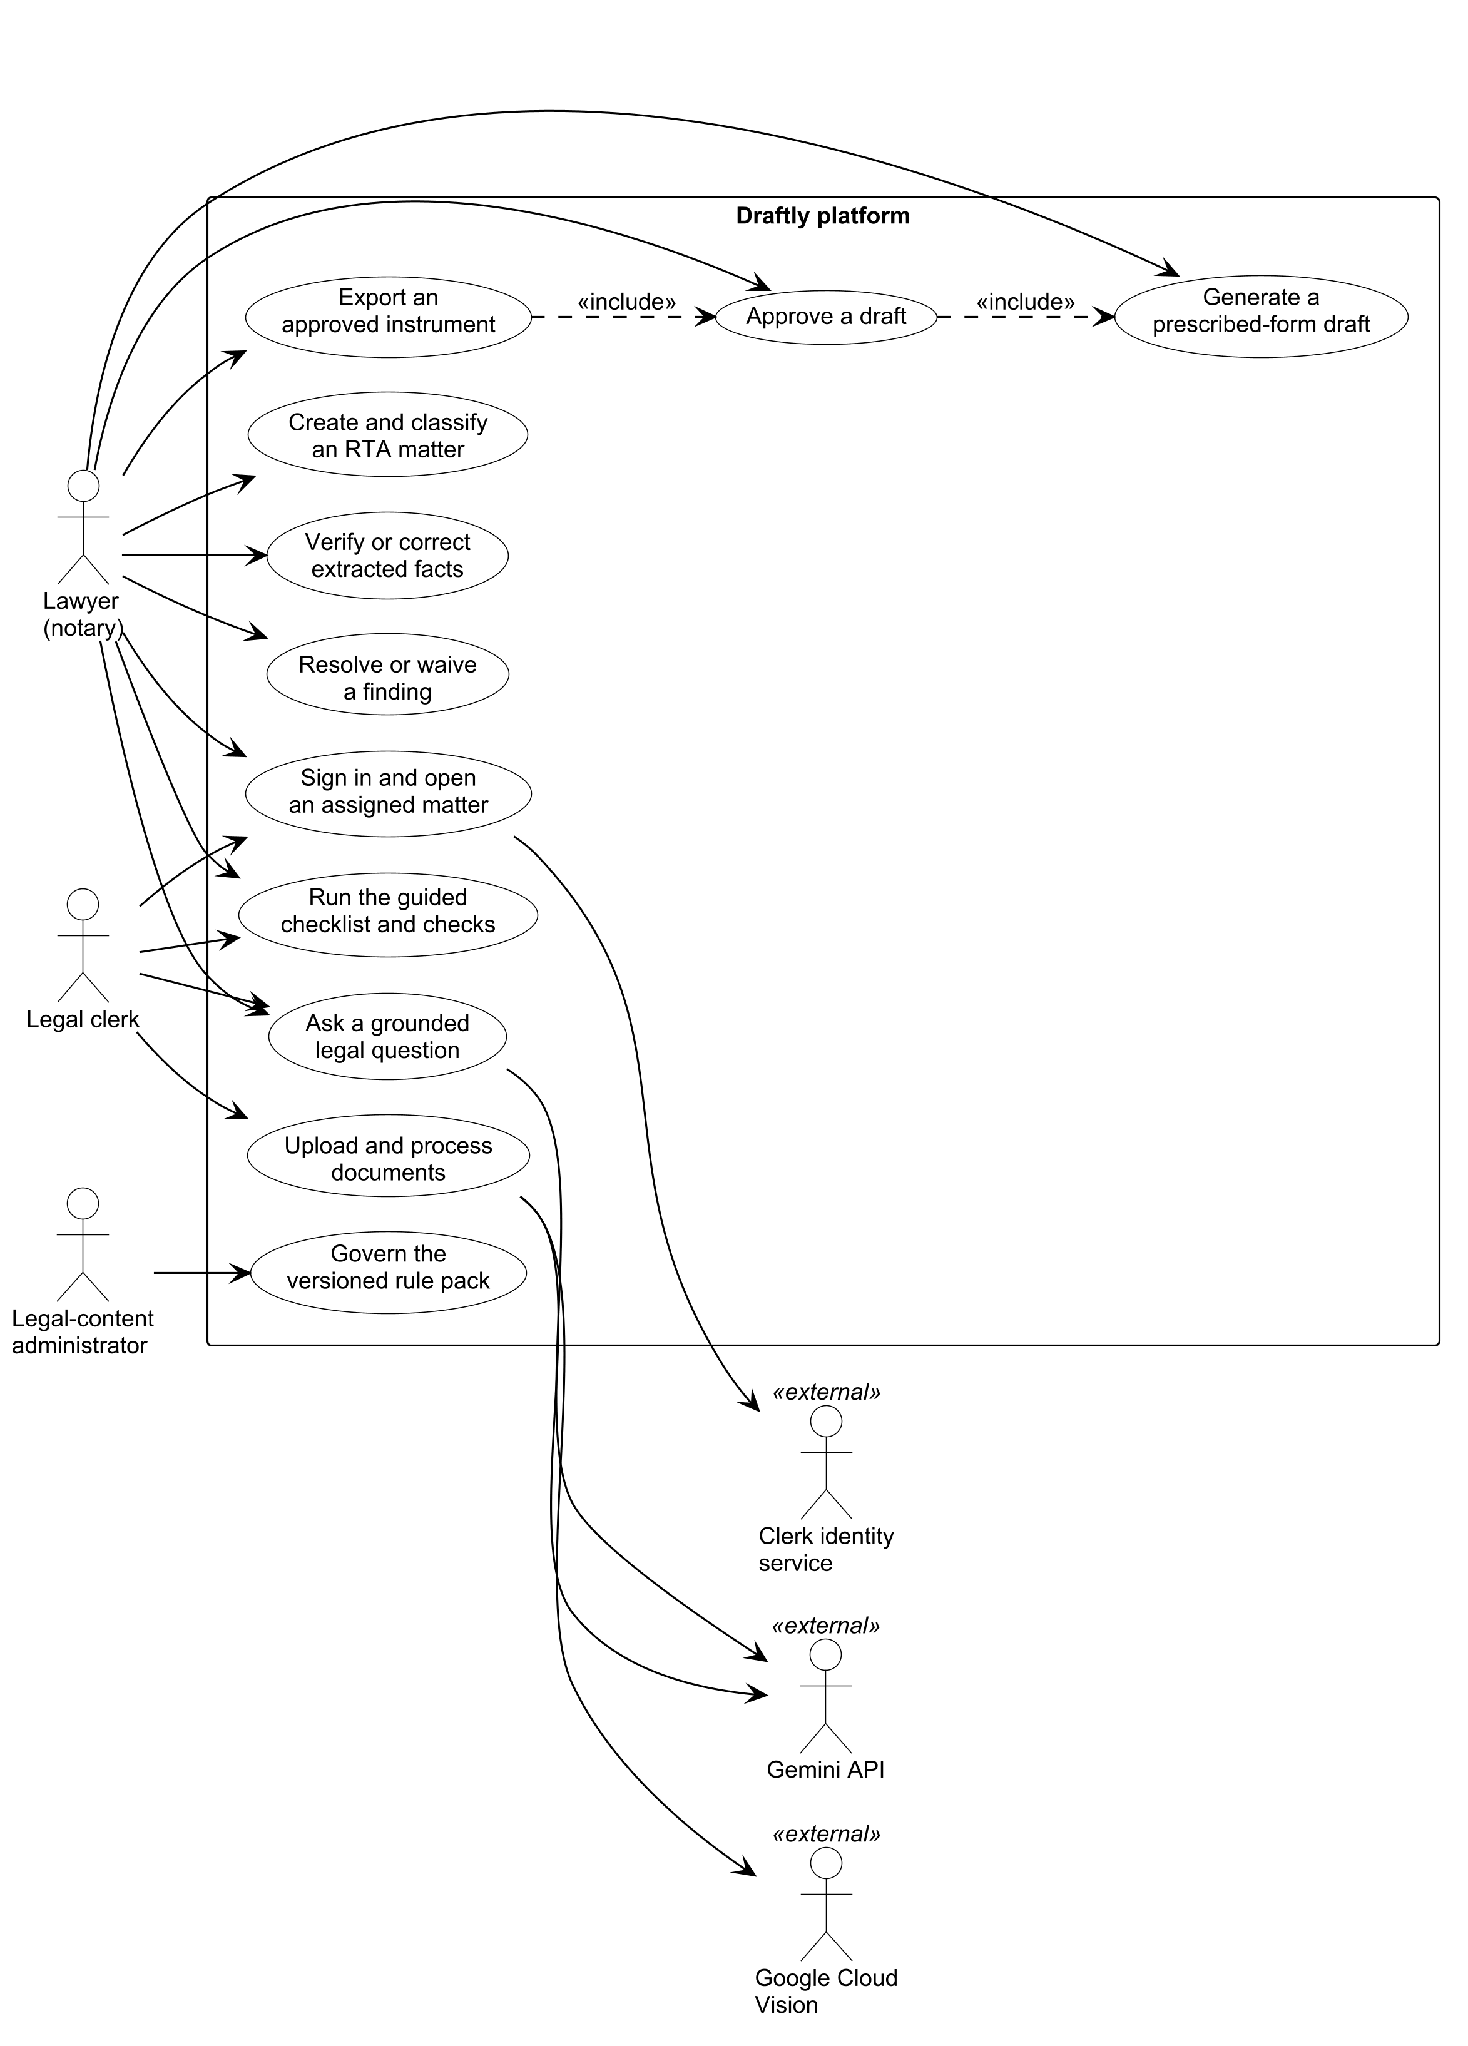
\includegraphics[width=\linewidth,height=5in,keepaspectratio]{figures/report-fig-01-use-cases.png}
\caption{Main use cases and human authority in the Draftly workbench. This is a system-design view.}
\end{figure}

The principal quality requirements follow from this authority boundary. Organisation and matter isolation must be enforced on the server. Original evidence must remain immutable; corrections create new fact versions. Machine confidence cannot make a value verified, and a later correction must invalidate dependent work. Research must return cited material or state that authority is insufficient. The system records material mutations in an append-only, hash-chained audit log. These are engineering requirements tested at the service and database layers; they do not certify any legal answer or document wording.


\subsection{System Design}

\subsubsection{Architecture}

Draftly uses a Next.js browser workbench and a FastAPI backend arranged as domain modules. The backend stores matter data in self-hosted PostgreSQL on the VPS and processes asynchronous work through an outbox worker. It calls a separate retrieval service over the internal network. The hosted deployment uses Caddy for TLS and routing, Clerk for sign-in, a BM25 lexical index in the retrieval container, and Gemini for research-answer composition. Its source files currently use a VPS volume, and MinIO is the planned object-storage service. Document extraction remains on a stub provider in that deployment. Its connected matter screens read and write persistent API data. Fig. 2 shows this deployment and marks the MinIO addition separately; the research experiment evaluated different retrieval combinations [27]–[31].


\begin{figure}[H]
\centering
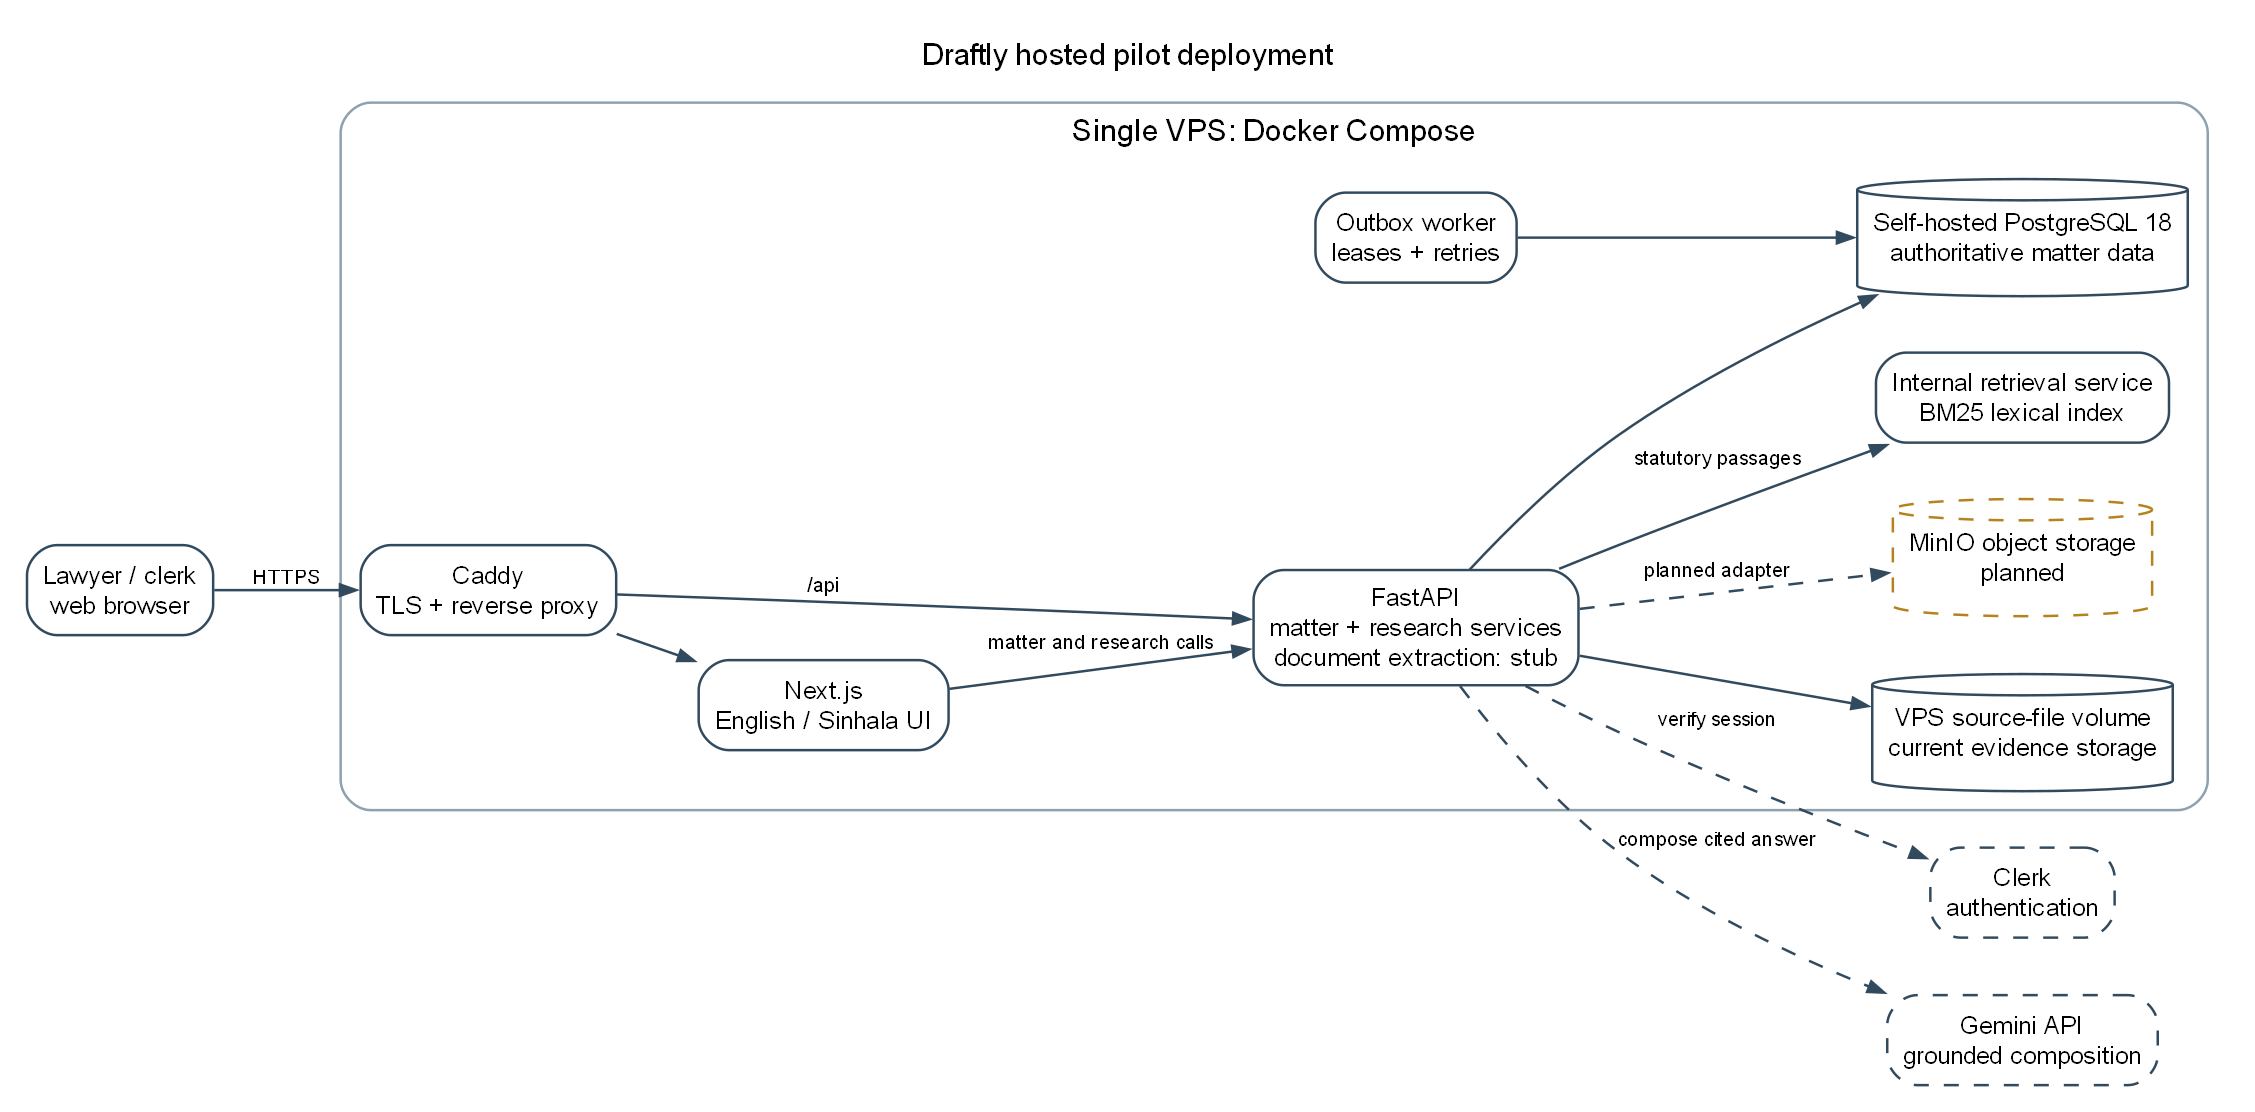
\includegraphics[width=\linewidth,height=5in,keepaspectratio]{figures/deployment-demo.png}
\caption{VPS deployment with self-hosted PostgreSQL and current source-file storage. The dashed MinIO connection is planned; extraction is stubbed and the internal retrieval index is lexical.}
\end{figure}

The domain modules follow a fixed dependency direction: an API router calls an application service, that service applies domain policy through a port, and infrastructure adapters provide storage or external integrations. This permits a rule about verification or approval to be tested without depending on a browser screen. It also prevents a retrieval or model response from writing an authoritative fact directly.


\subsubsection{Logical and Process Views}

A Matter scopes Parties, SourceFiles, candidate ExtractedFacts, EvidenceReferences, ReviewDecisions, Findings, and AuditEvents. A candidate is supported by a file hash and location in the evidence. A correction supersedes the previous fact instead of silently replacing it. ResearchClaims link to ResearchCitations; requirements and checks are instantiated from a versioned RulePack. The conceptual associations appear in Fig. 3. The diagram also includes the draft, approval, and export records that connect verified matter facts to later lawyer actions.


\begin{figure}[H]
\centering
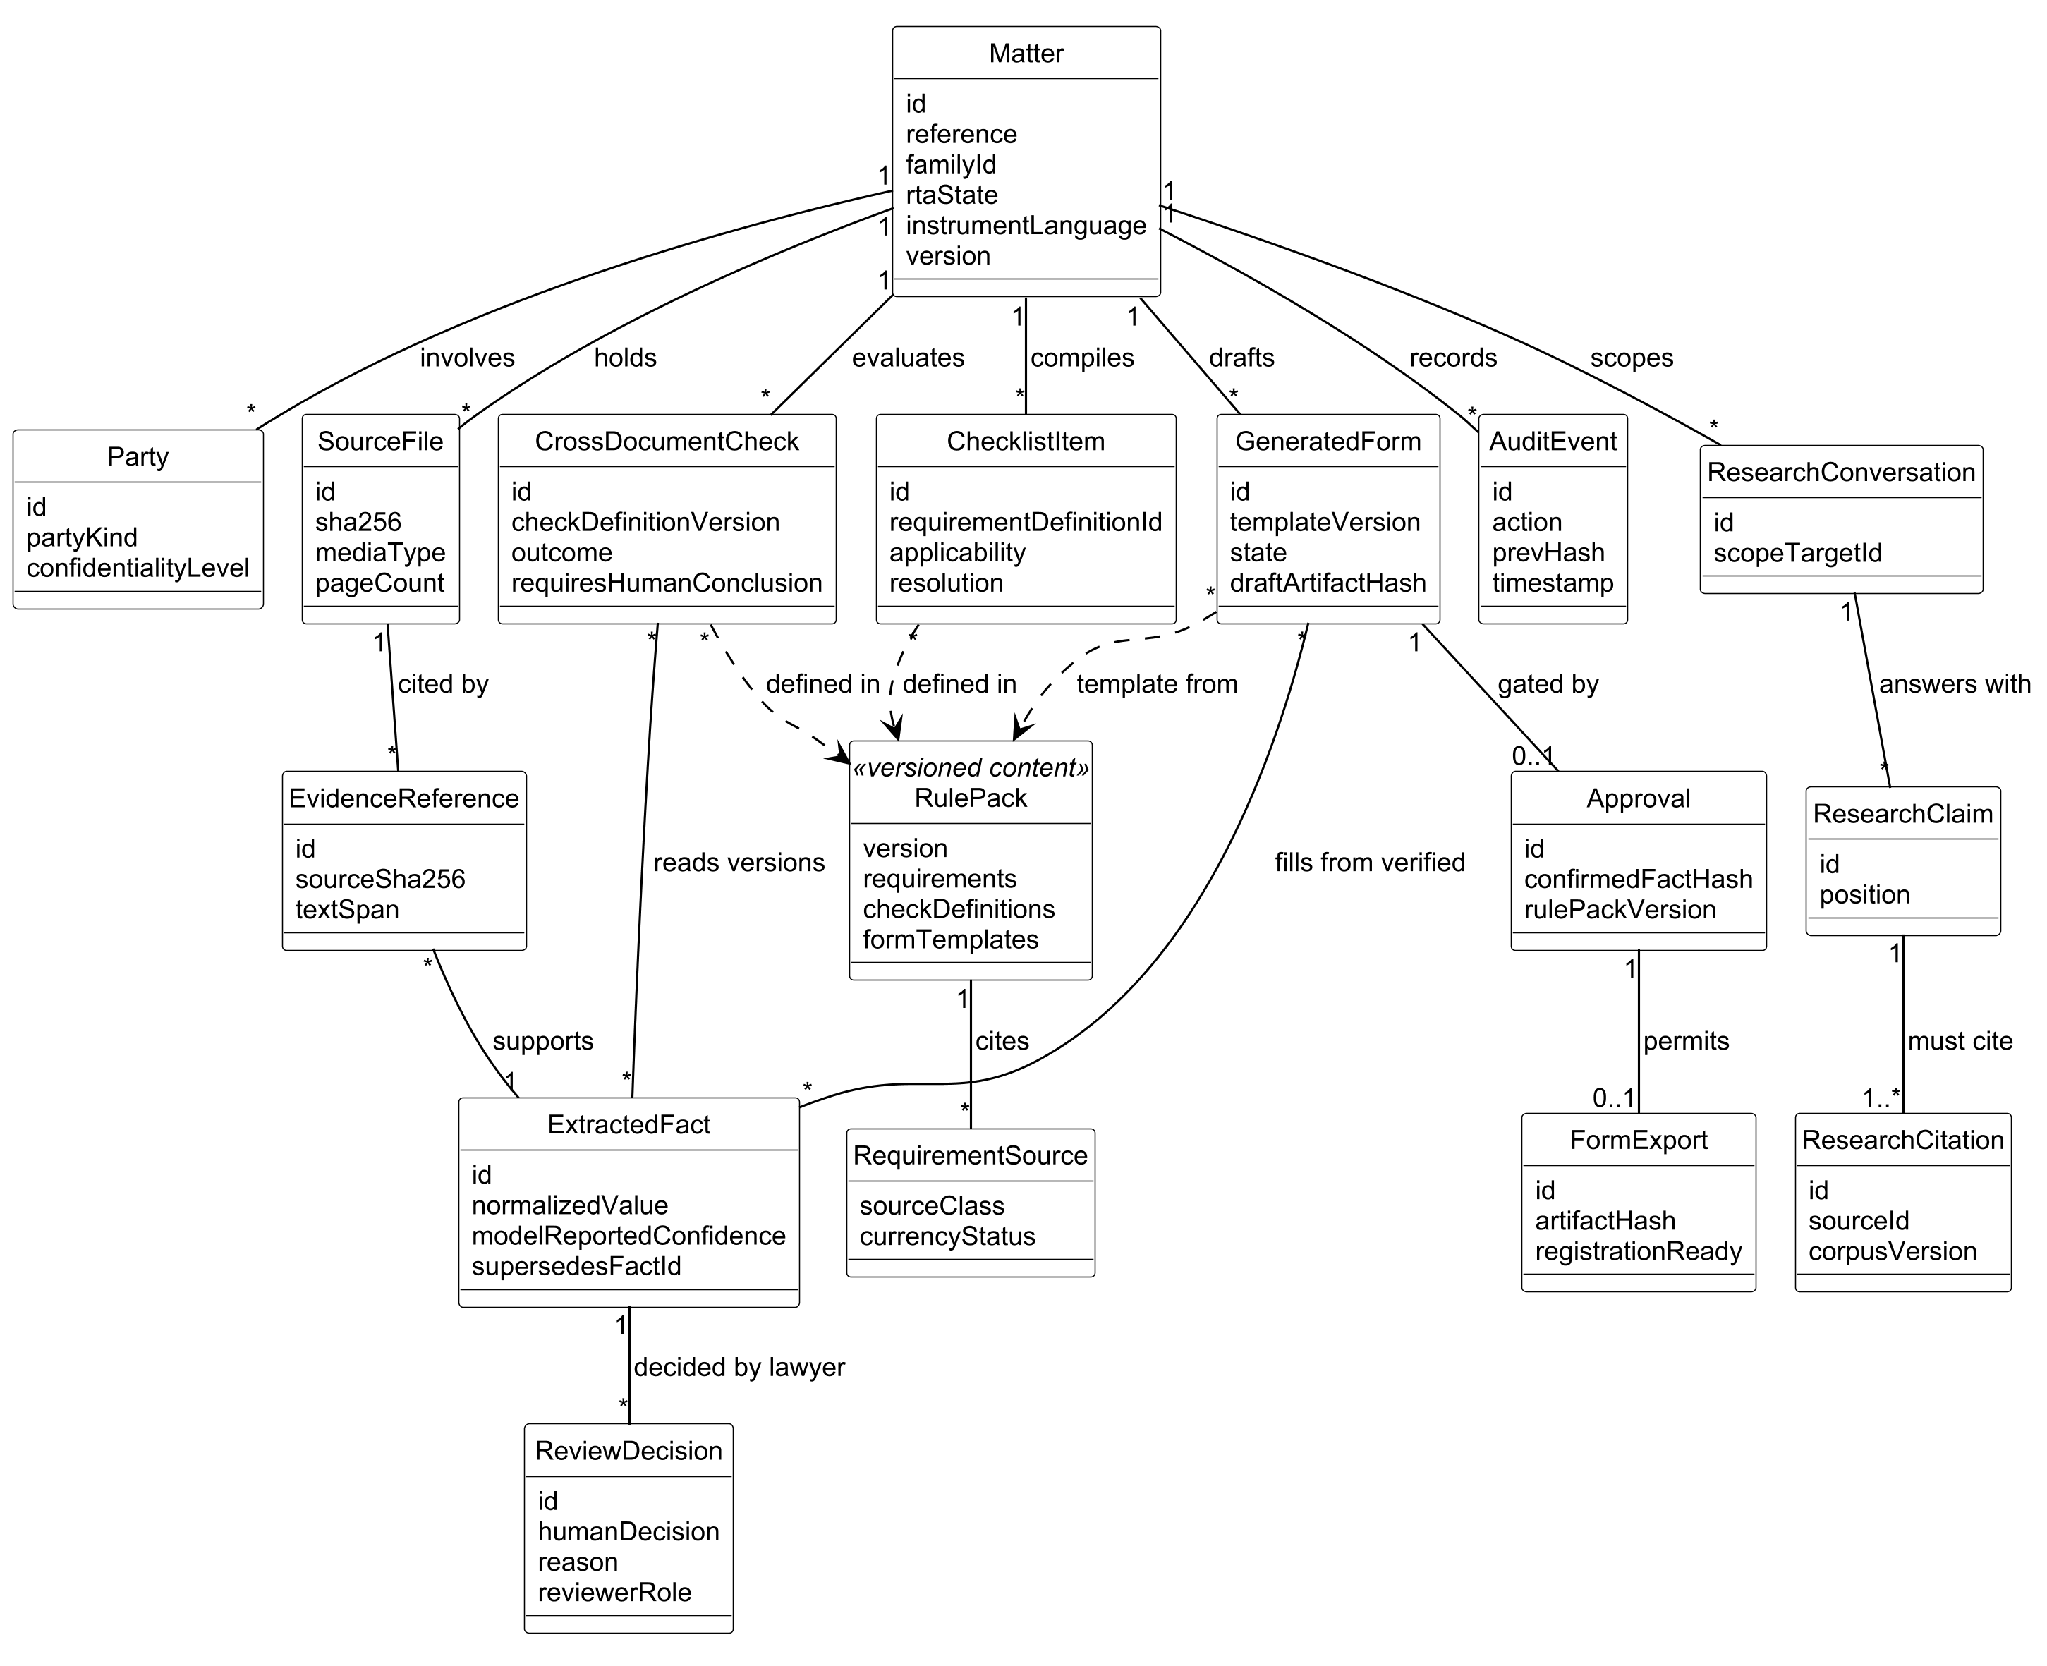
\includegraphics[width=\linewidth,height=5in,keepaspectratio]{figures/report-fig-03-domain-classes.png}
\caption{Conceptual classes connecting a matter, evidence, review decisions, governed rules, research citations, and downstream controls.}
\end{figure}

Fig. 4 follows a transfer matter. A user creates the matter and supplies documents; processing produces candidates; the lawyer verifies or corrects them; rule-pack checks surface mismatches and missing evidence; and the lawyer records a resolution. The draft, approval, and export stages apply explicit prerequisites and preserve the lawyer's decision in the matter record.


\begin{figure}[H]
\centering
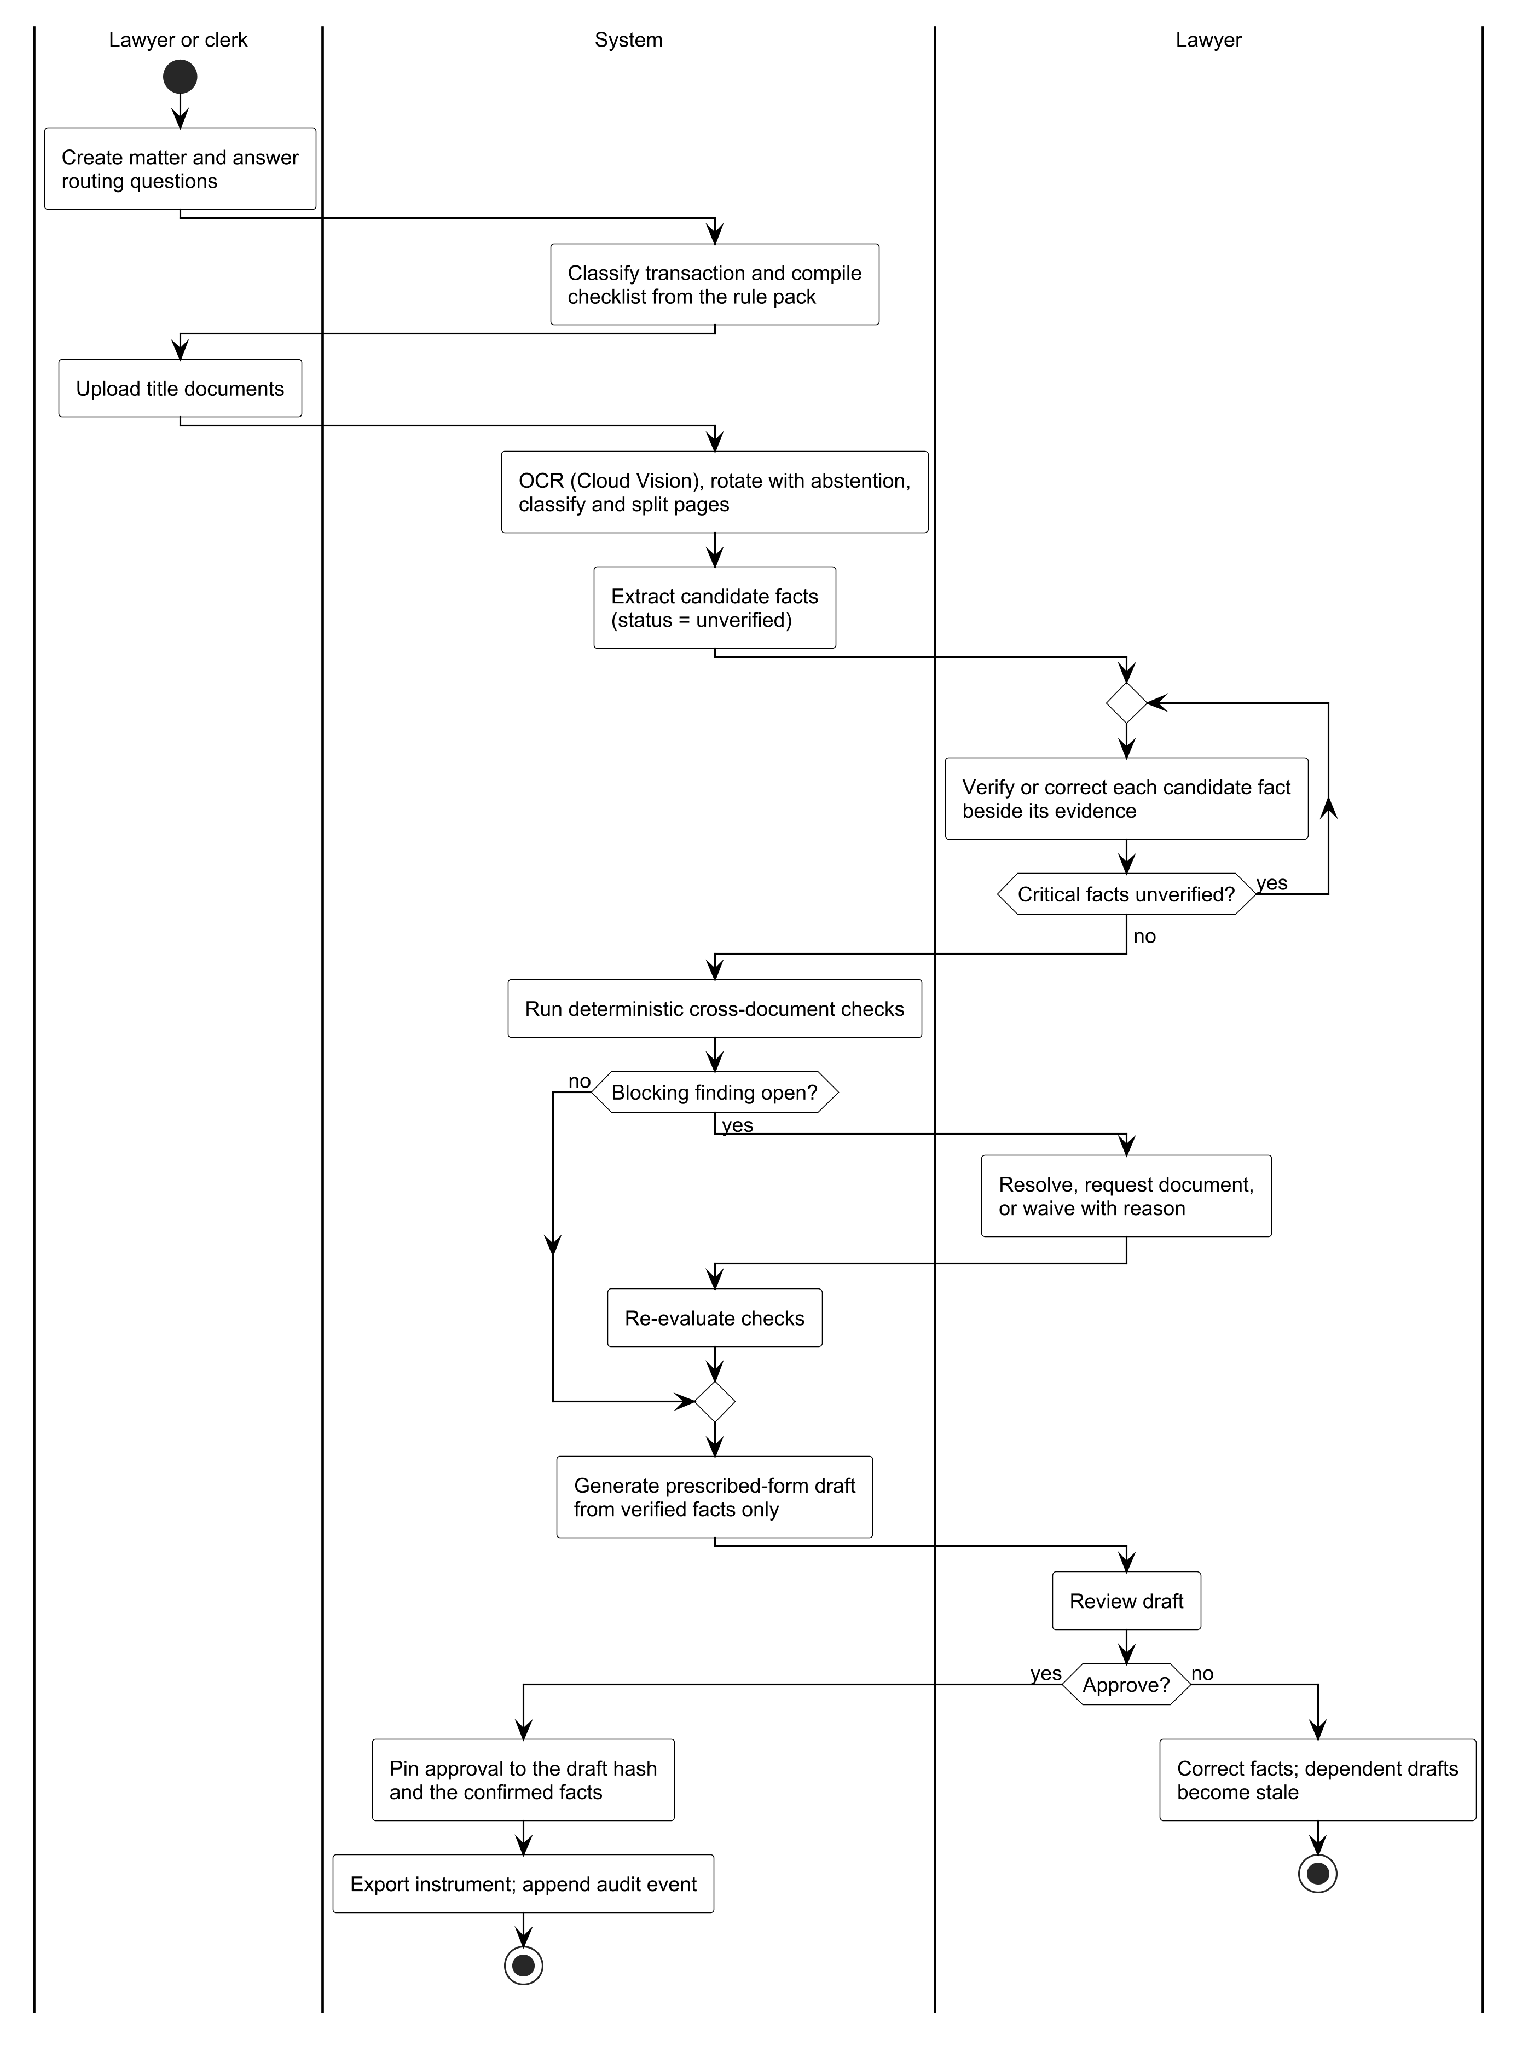
\includegraphics[width=\linewidth,height=5in,keepaspectratio]{figures/report-fig-04-rta-transfer-activity.png}
\caption{Designed Registration of Title Act matter flow, from evidence review through checks, drafting, and lawyer approval.}
\end{figure}

\subsection{Database Design}

The database separates source evidence, derived candidates, lawyer decisions, governed content, and audit records. Fig. 5 shows the core relations. A source file carries a content hash; a derived file points to its origin, preserving the original. An extracted fact records source provenance and version. Review decisions store who accepted or corrected a value and the reason. Findings remain separate from facts so a detected mismatch cannot itself resolve the matter. Audit events link to the preceding event hash. Optimistic version fields reject stale writes, and the transactional outbox lets work resume after a worker interruption. The database and migrations were tested on PostgreSQL rather than only on an in-memory substitute [29].


\begin{figure}[H]
\centering
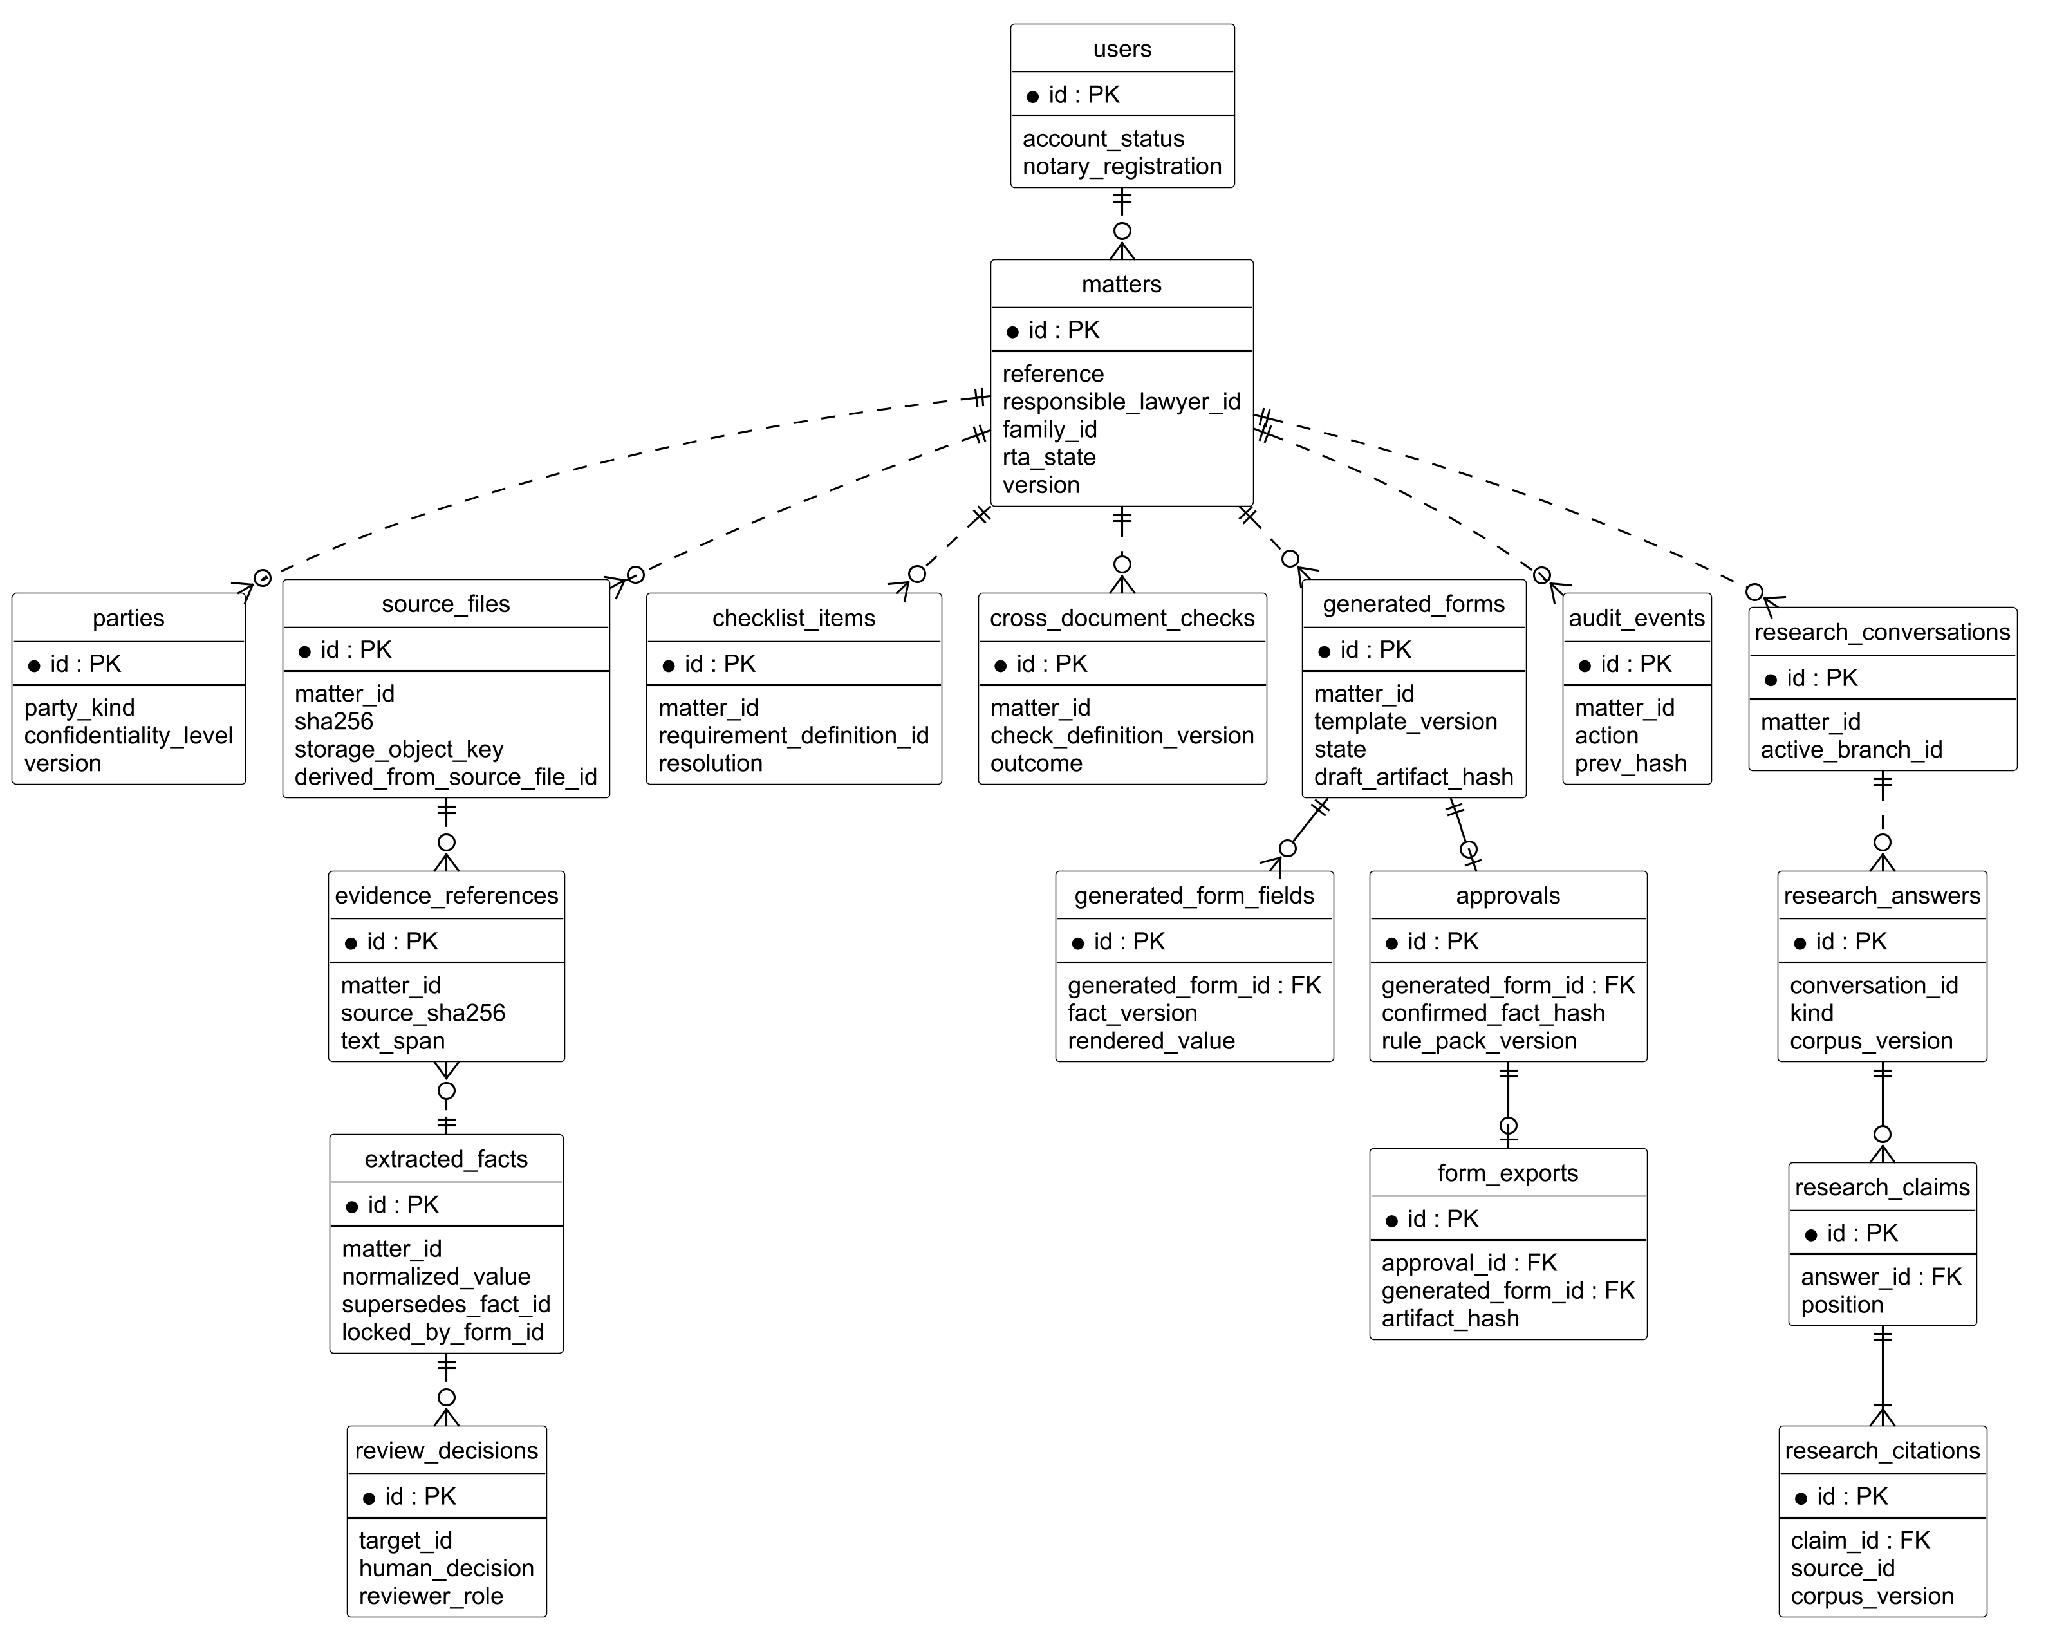
\includegraphics[width=\linewidth,height=5in,keepaspectratio]{figures/report-fig-05-core-er.png}
\caption{Core matter and research entity relationships. Solid lines represent database foreign keys; dashed lines represent logical references.}
\end{figure}

The research data has a different storage pattern. Structured Acts, sections, provisions, and typed edges are held in versioned JSON Lines with a corpus fingerprint and per-file hashes. The retrieval index uses SQLite FTS5 for lexical search. A changed corpus fingerprint causes a rebuild rather than reusing an old index. This separation lets the paper's frozen benchmark be inspected without treating provisional research labels as authoritative matter data.


\subsection{Machine Learning and Data Science System Design}

\subsubsection{Statutory Corpus and Benchmark}

The research corpus contains 52 principal enactments and 60 amending Acts, 4,557 sections, 17,854 sub-section provisions, and 6,346 typed edges. Edges encode definitions, exceptions, qualifications, procedural requirements, cross-references, and amendments. The 16 Law College examination papers were split into 667 atomic questions. After eligibility review and two-agent annotation, 50 statute-only questions in 40 matters formed the scored benchmark, with 84 distinct provisions proposed as indispensable. A deterministic validator checked section identifiers and verbatim excerpts. This verifies that a label points to text in the frozen corpus; it does not establish that the provision is legally indispensable. Fig. 6 shows the proposed annotation process and its planned human legal review. The three-attorney validation shown there has not run.

\begin{figure}[H]
\centering
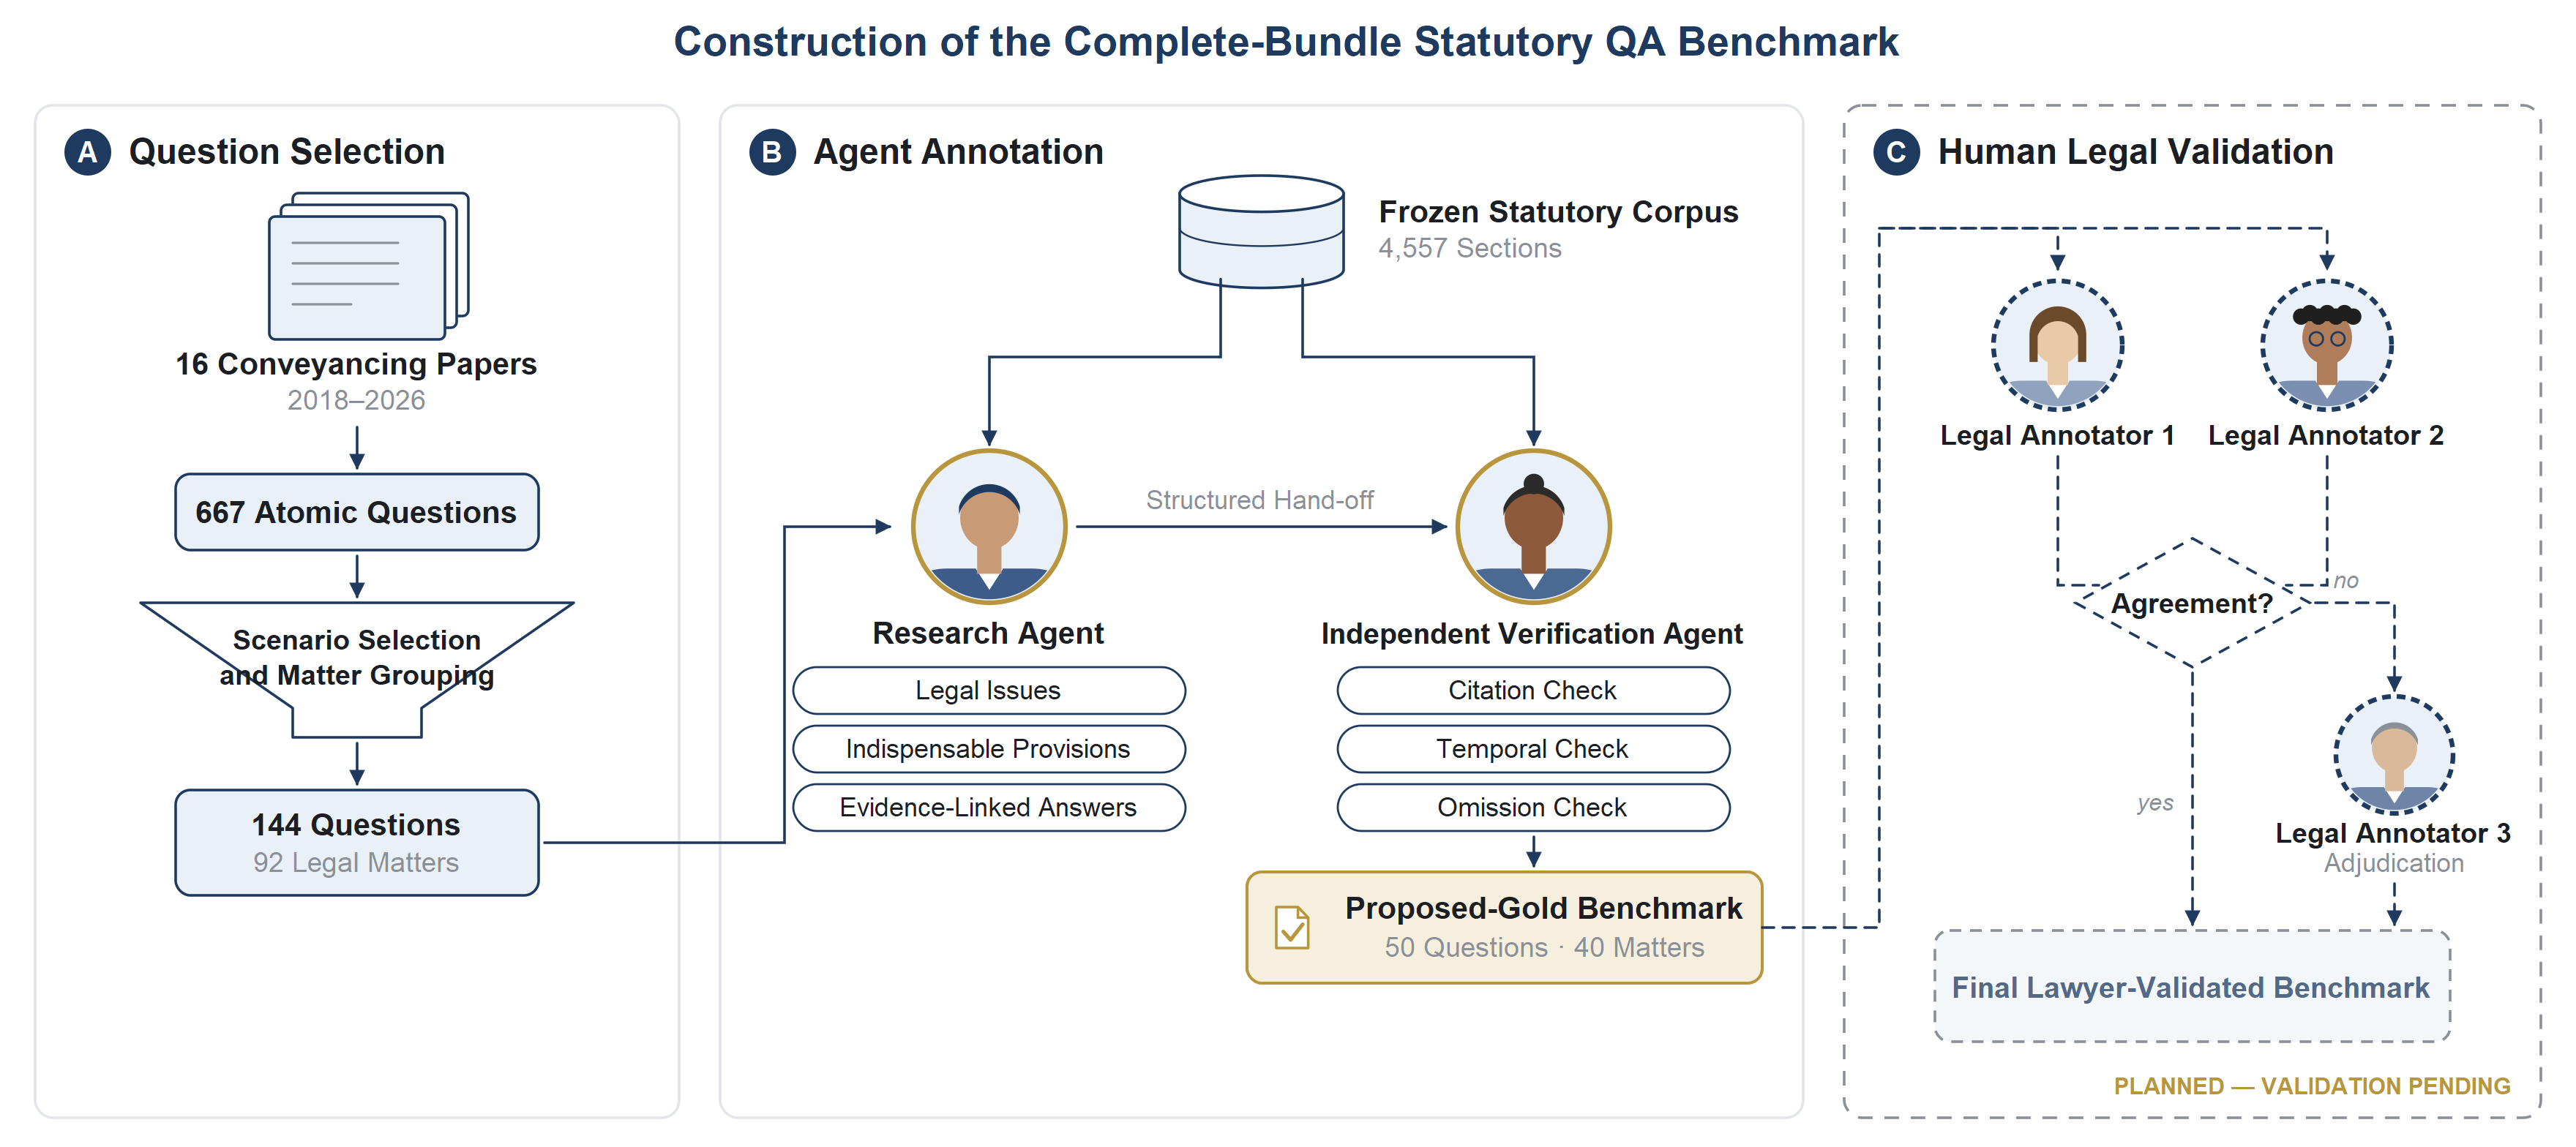
\includegraphics[width=\linewidth,height=3.8in,keepaspectratio]{figures/research-benchmark-construction-preview.png}
\caption{Benchmark construction from examination questions to proposed indispensable provisions. The lawyer annotation and adjudication stage is planned and remains pending.}
\end{figure}


\subsubsection{Retrieval and Grounded Research}

Seven retrievers share the same questions and corpus. The lexical systems use ordinary and field-weighted BM25. Dense retrieval ranks overlapping windows of long sections. Hybrid retrieval fuses lexical and dense ranks. A further variant reranks candidates with a cross-encoder. Hierarchical retrieval first selects likely Acts, while the structure-aware variant expands selected section seeds along typed edges and applies a temporal filter. Fig. 7 shows the corpus, tested alternatives, and the all-or-nothing evaluation rule. It is a research diagram, not a diagram of the currently deployed lexical index.


\begin{figure}[H]
\centering
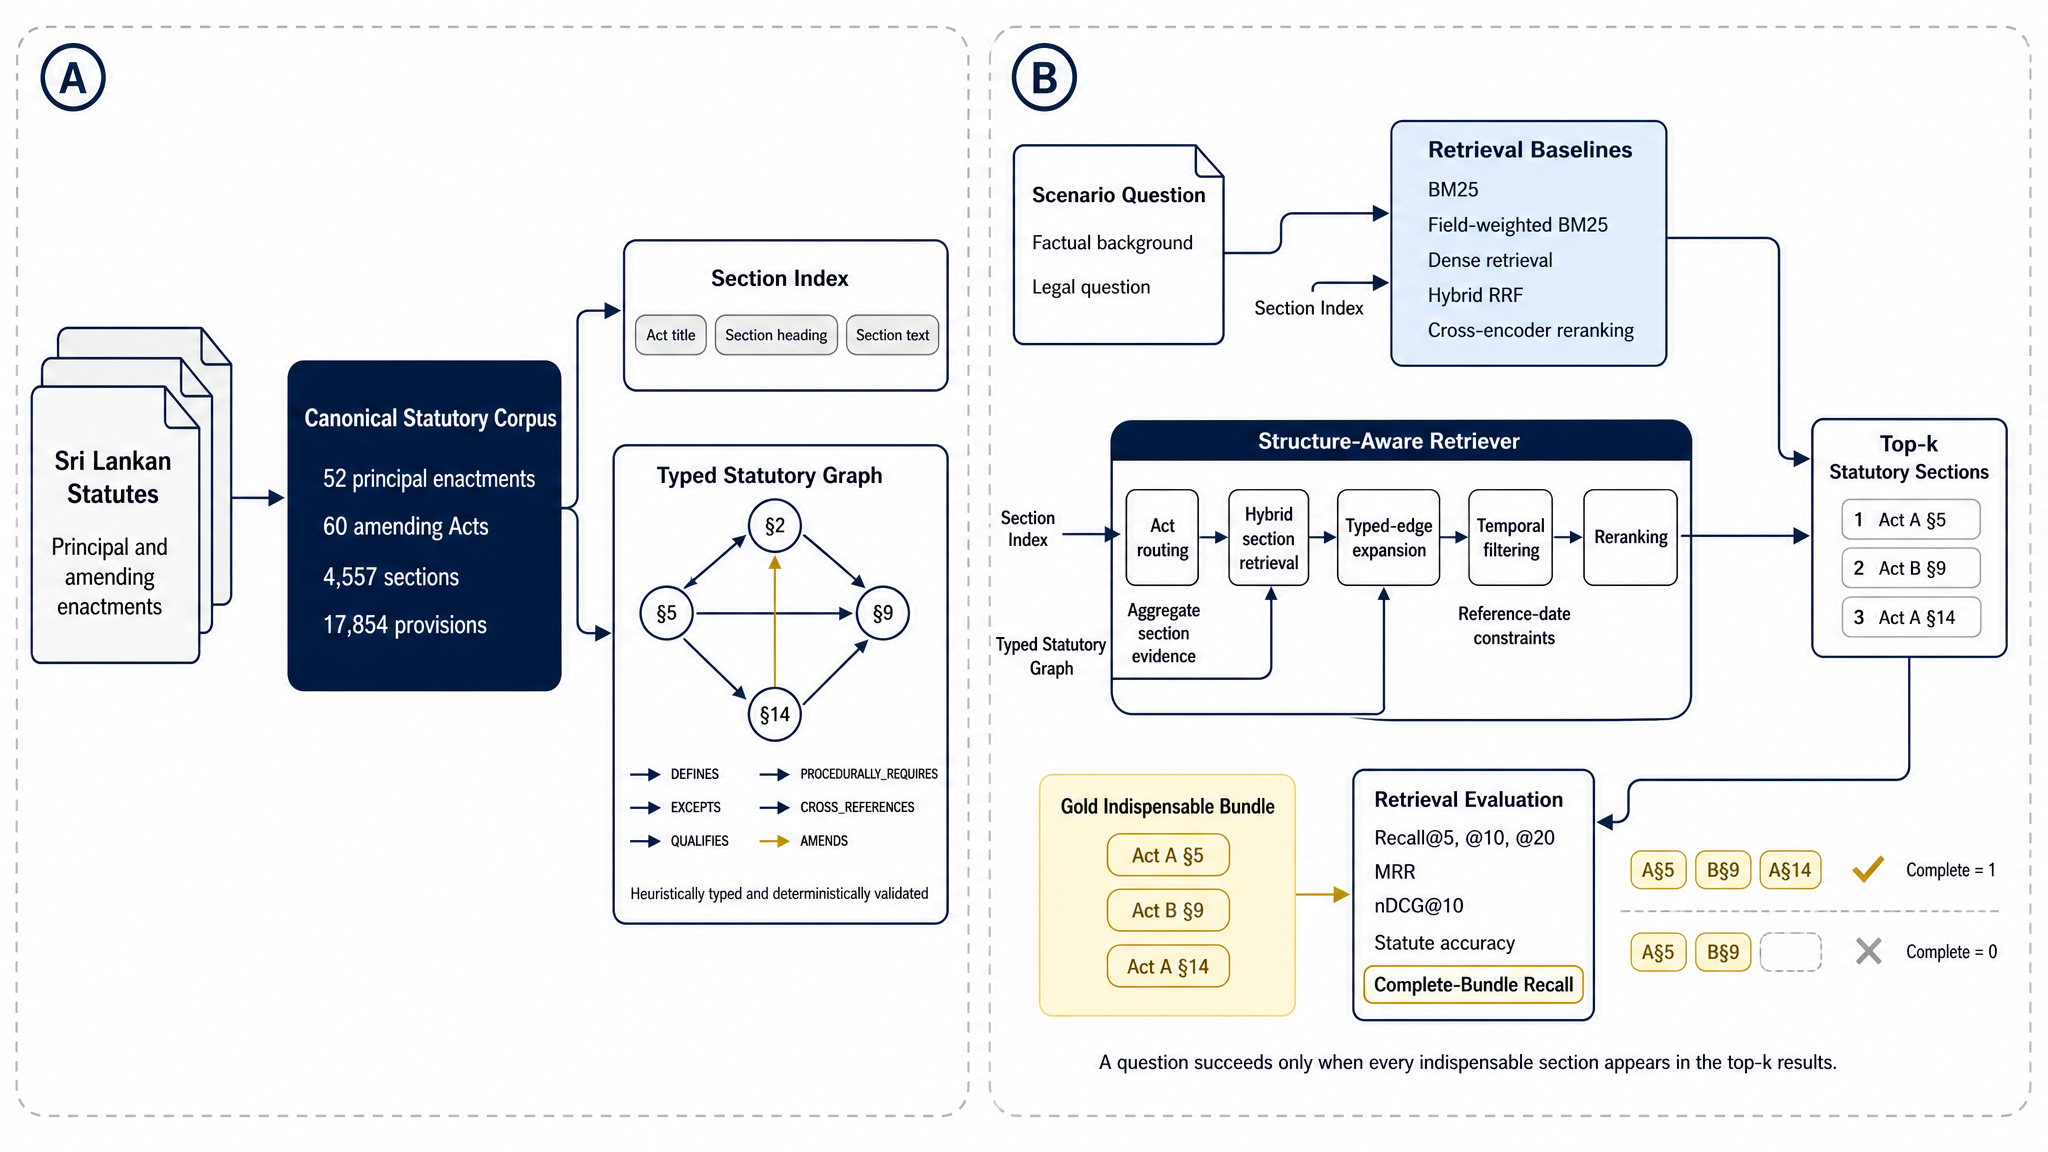
\includegraphics[width=\linewidth,height=5in,keepaspectratio]{figures/research-corpus-retrieval-paperbanana.png}
\caption{Frozen statutory corpus and retrieval systems evaluated in the research paper; the proposed indispensable bundle defines a complete result.}
\end{figure}

The research-answer path composes an answer from retrieved passages and requires each emitted claim to name a returned authority identifier. It rejects claims with citations outside that returned set and abstains when the engine supplies no usable authority. The platform also turns retrieval timeouts into an insufficient-authority response. These checks limit unsupported output but do not prove the legal correctness of an answer; the answer-generation stage has not received attorney scoring.


\subsubsection{Case Law and Document Reading}

A deterministic headnote reader recovered a verbatim rule from 3,521 of 3,703 reported judgments. Cases it could not parse, and unreported judgments, entered a bounded model-assisted route using Llama 3.1 8B through NVIDIA NIM. That route required a quotation occurring verbatim in the judgment and rejected section references outside a closed catalogue [32], [33]. A held-out evaluation found that the accepted output was still below the project's usability threshold, so extracted rules remain unverified. Case-law ranking is not part of the scored statutory benchmark.


For scanned matter documents, the research team compared OCR engines on multilingual pages and chose Google Cloud Vision for the pipeline design [30]. The designed pipeline checks page quality and orientation, groups pages into logical documents, and produces string-valued candidate fields for human review. Fig. 8 separates the current hosted source-file volume and stub extraction from the designed OCR and classification path. MinIO is marked as planned object storage; Laya is an evaluation candidate for classifying OCR text after extraction. Sinhala and Tamil character recovery and page rotation were observed, while a field-level accuracy study remains a separate evaluation task. Lawyer review is the boundary between candidate output and verified matter facts.

\begin{figure}[H]
\centering
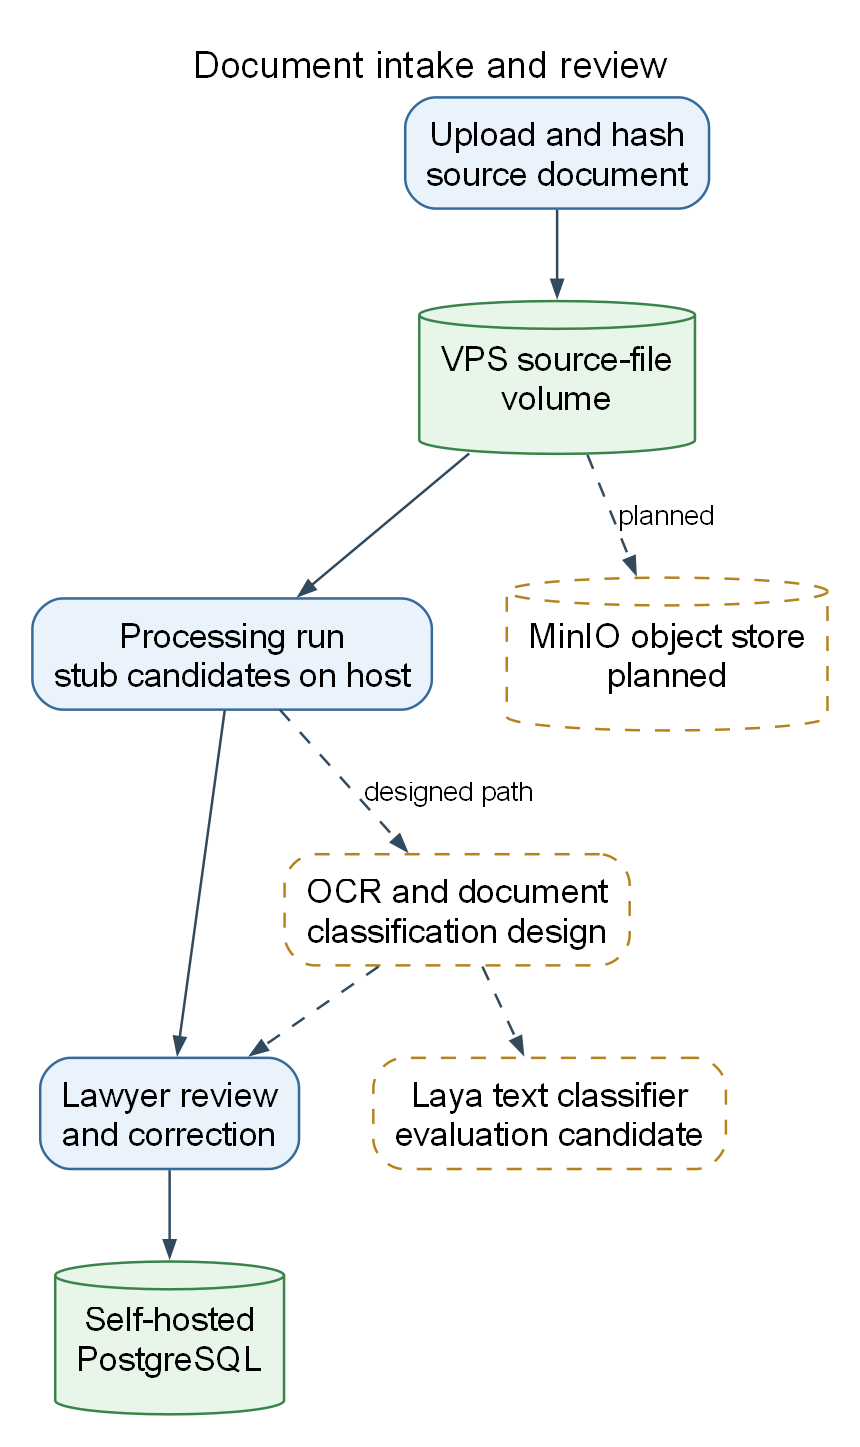
\includegraphics[width=\linewidth,height=5in,keepaspectratio]{figures/document-processing-current-target.png}
\caption{Document intake and review. Solid paths show the hosted VPS volume, stub processing, lawyer review, and self-hosted PostgreSQL; dashed paths mark planned MinIO storage and the OCR and classification candidates.}
\end{figure}


\section{System Implementation}

\subsection{Implementation Procedure}

The research code is written in Python and uses deterministic corpus builds, content hashes, versioned experiment configurations, and stored per-question rankings. Its retrieval service exposes a bounded search interface to the platform. The benchmark systems were run on a laptop processor, with identical test questions and corpus inputs across configurations. Corpus and split fingerprints, software versions, and run manifests were recorded so that a score refers to one frozen build. The public release contains the benchmark questions and provisional labels with a small evaluator; it does not include the frozen full-text corpus or all retrieval implementations, so publication of the labels alone does not reproduce the paper's experiment.


The platform backend uses FastAPI, SQLAlchemy, Alembic and PostgreSQL; its frontend uses Next.js, React and TypeScript [27]–[29]. Domain rules are implemented in services rather than in screen components. Server-side user scoping protects matters. Facts are promoted through explicit review decisions, while the content-governance service records where each workflow requirement came from. An outbox worker claims jobs with leases and retries, and a hash-chained audit log records material actions. The frontend provides matter, document, facts, workflow, checks and research views in English and Sinhala. It also includes intake, party records, approval and export controls, practice operations, account and billing functions. A Docker Compose stack hosts the API-backed workbench on one virtual private server. A research-service failure produces an insufficient-authority response. The single-server and current provider settings limit claims about production readiness.


The Registration of Title Act rule pack is versioned data. Its exported contract records nine transaction families, 33 matter subtypes, 145 checklist requirements, 25 deterministic checks, 52 document classes, and 32 form templates. Each requirement identifies a source class so that an Act obligation can be distinguished from registry operations or professional practice. Template bindings use verified matter facts, while preflight checks and approval records preserve a reviewable drafting trail.


\begin{table}[H]
\centering
\caption{Implemented areas and their demonstrated boundary.}
\fontsize{9.5}{11}\selectfont
\begin{tabularx}{\linewidth}{>{\RaggedRight\arraybackslash}X|>{\RaggedRight\arraybackslash}X|>{\RaggedRight\arraybackslash}X}
\toprule
\textbf{Area} & \textbf{Demonstrated work} & \textbf{Boundary} \\
\midrule
Legal corpus and benchmark & Deterministic build, proposed provision labels and seven-system comparison & Attorney validation pending \\
Research interface & Retrieved passages, citation identifiers and abstention on unavailable authority & Answer correctness not lawyer-scored \\
Matter workbench & Persistent matter records, evidence-linked candidates, rule-pack steps, findings and audit & Real-client use not approved \\
Document processing & Multilingual OCR pipeline and engine comparison in research & Deployed extraction is stub; field accuracy unmeasured \\
Draft controls & Form bindings, review, approval and export records & Prerequisite refusal rules tested \\
\bottomrule
\end{tabularx}
\end{table}

\subsection{Materials}

The research corpus was assembled from Sri Lankan statutes and amending Acts available through official and republisher sources. Reported judgments came from the CommonLII archive of the New Law Reports and Sri Lanka Law Reports; official court material supplied unreported judgments. The benchmark questions came from sixteen Sri Lanka Law College conveyancing examinations, which were structured into 667 atomic questions. The rule pack cites ten governed sources across law, regulation, registry operations, local-authority operations, professional practice, product rules, and material awaiting verification. Scanned conveyancing documents used in document-reading experiments contain personal information, so this report gives aggregate characteristics only and does not reproduce their pages, identifiers or OCR overlays. Synthetic matter data supplies the platform demonstration and interface figures.


\begin{table}[H]
\centering
\caption{Materials and their role in the project.}
\fontsize{9.5}{11}\selectfont
\begin{tabularx}{\linewidth}{>{\RaggedRight\arraybackslash}X|>{\RaggedRight\arraybackslash}X|>{\RaggedRight\arraybackslash}X}
\toprule
\textbf{Material} & \textbf{Scale or format} & \textbf{Use and restriction} \\
\midrule
Statutes and amendments & 52 principal and 60 amending Acts in the frozen benchmark corpus & Section retrieval and typed relationships; structural checks do not equal legal approval \\
Law College questions & 16 papers, 667 atomic questions, 50 scored questions & Proposed benchmark labels; attorney validation pending \\
Reported judgments & 3,703 CommonLII full-text judgments & Headnote rule recovery; outputs unverified \\
Unreported judgments & 5,474 Supreme Court and Court of Appeal documents & Bounded extraction and linking; no lawyer-verified rule set \\
Registration of Title Act rule pack & Ten governed sources, version 1.0.0 & Checklist, checks and form bindings \\
Matter documents & Scanned PDF and image files held outside public outputs & OCR research in aggregate only; no client material in figures \\
\bottomrule
\end{tabularx}
\end{table}

\subsection{The Algorithms}

The first algorithm tested whether statutory relationships improve the retrieval of complete provision sets. It begins with lexical and dense rankings, routes the query to a small set of Acts, and takes high-ranked sections as seeds. It then adds sections linked by enabled edge types, removes material outside the question's reference date, and reranks the candidates. Fig. 9 gives the essential procedure without implementation code. The temporal step measures one useful control, although the tested edge expansion did not improve complete recall against the strongest comparison methods.


\begin{figure}[H]
\centering
\fbox{\begin{minipage}{0.95\linewidth}\ttfamily\fontsize{8}{10}\selectfont
Input: question q, reference date d, section corpus S, typed edges E\\L = BM25(q, S); D = dense\_search(q, S)\\A = select\_likely\_Acts(q, L, D)\\Seeds = top\_sections(rank\_fusion(L, D), within=A)\\Candidates = Seeds union typed\_neighbours(Seeds, E)\\Candidates = keep\_in\_force(Candidates, d)\\Return rerank(q, Candidates)[:20]
\end{minipage}}
\caption{Structure-aware retrieval tested in the statutory benchmark}
\end{figure}

The second procedure is the research answer boundary. Returned passages become an allowlist of authority identifiers. A generated claim is retained only if it points to an identifier in that allowlist; failure to retrieve material or to retain a cited claim results in an abstention. Fig. 10 shows that control. It is a provenance check rather than a legal-validity test. A lawyer still needs to inspect the cited provision and the proposed interpretation.


\begin{figure}[H]
\centering
\fbox{\begin{minipage}{0.95\linewidth}\ttfamily\fontsize{8}{10}\selectfont
Input: lawyer question q; retrieved passages P\\If retrieval fails or P is empty: return INSUFFICIENT\_AUTHORITY\\Allowed = \{p.authority\_id for p in P\}\\Claims = compose\_answer(q, P)\\Kept = [c for c in Claims if all(id in Allowed for id in c.citations)]\\If Kept is empty: return INSUFFICIENT\_AUTHORITY\\Store Kept and their cited passages as unverified research output\\Return Kept with citations for lawyer review
\end{minipage}}
\caption{Citation-identifier gate in the research answer path}
\end{figure}

\subsection{Main Interfaces}

The interface follows the order of a matter rather than opening with a general chatbot. A matter holds documents, facts, workflow steps, checks, research and activity history. Fig. 11 shows a July 2026 synthetic prototype of the fact-review view: candidates have status, confidence, source page and a separate verification action. The side-by-side evidence area makes it possible to compare conflicting values before a lawyer chooses one. This figure demonstrates interface design; it does not establish OCR accuracy or current live-screen fidelity.


\begin{figure}[H]
\centering
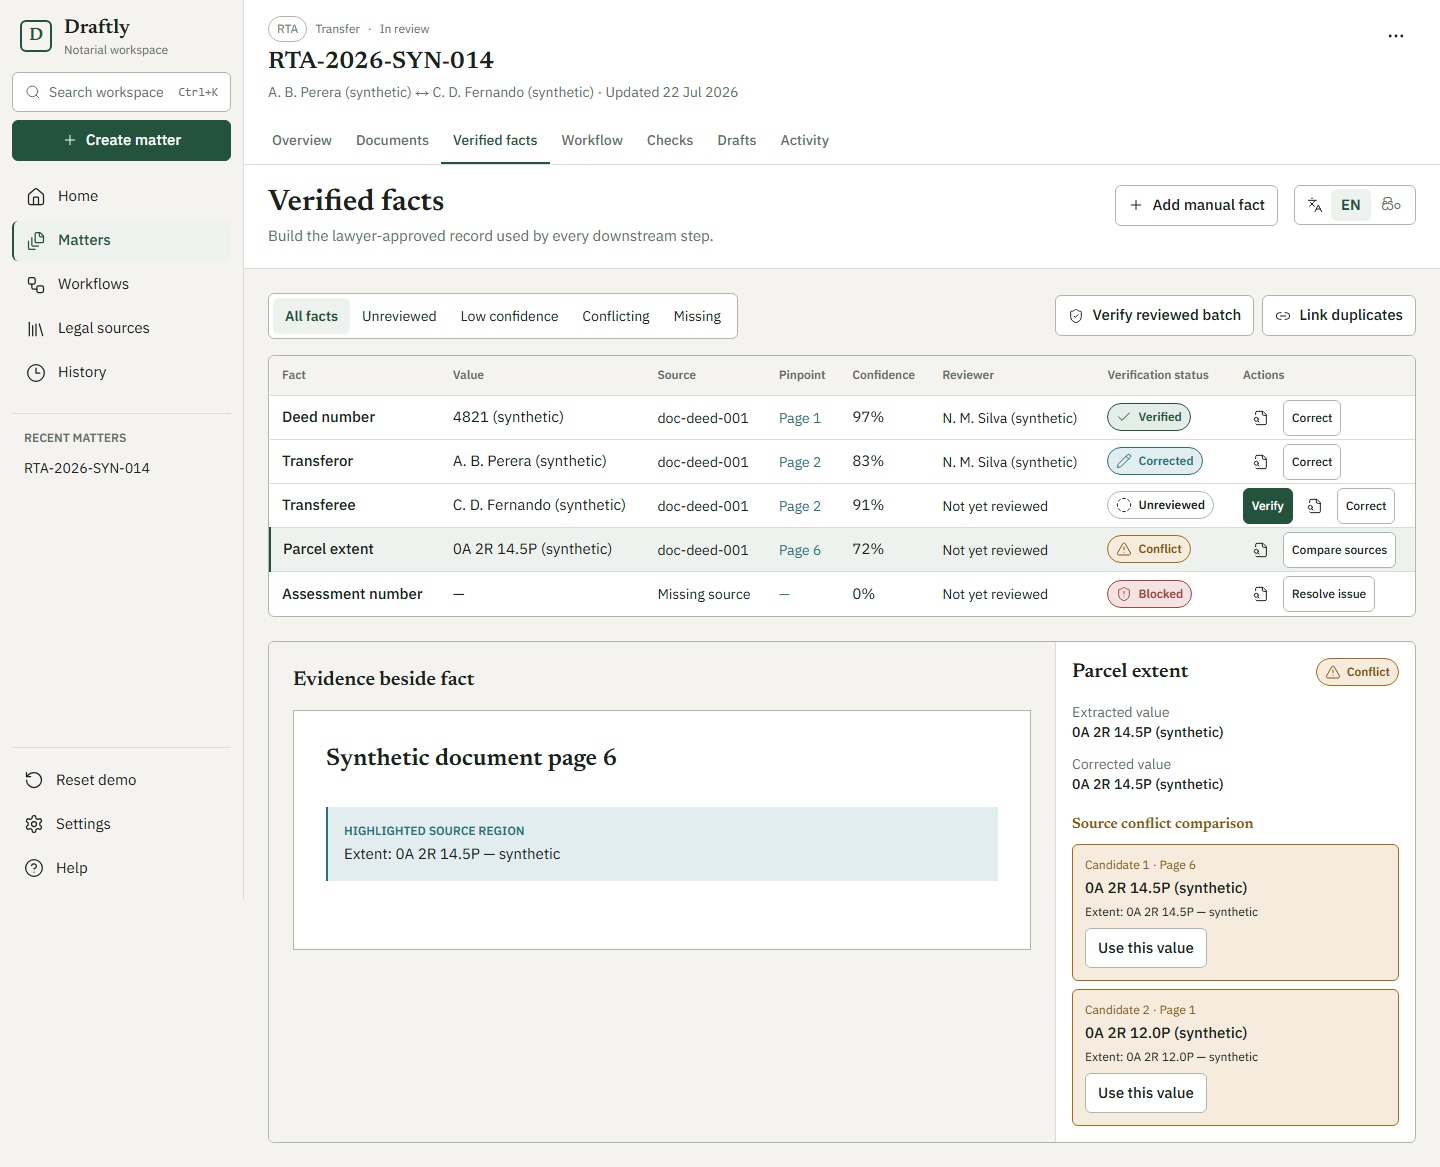
\includegraphics[width=\linewidth,height=5in,keepaspectratio]{figures/ui-prototype-fact-review.png}
\caption{Fact-review prototype with synthetic matter data, captured 22 July 2026. The evidence panel and verification controls are interface examples.}
\end{figure}

Fig. 12 shows the corresponding checks view. It groups missing evidence and conflicting particulars, states the source or affected fact, and offers a recorded resolution or waiver. A check finding is a prompt for review, not a determination of title. The screenshot is a dated synthetic prototype, so the final testing claims below are taken from the September backend and browser suites rather than inferred from the image.


\begin{figure}[H]
\centering
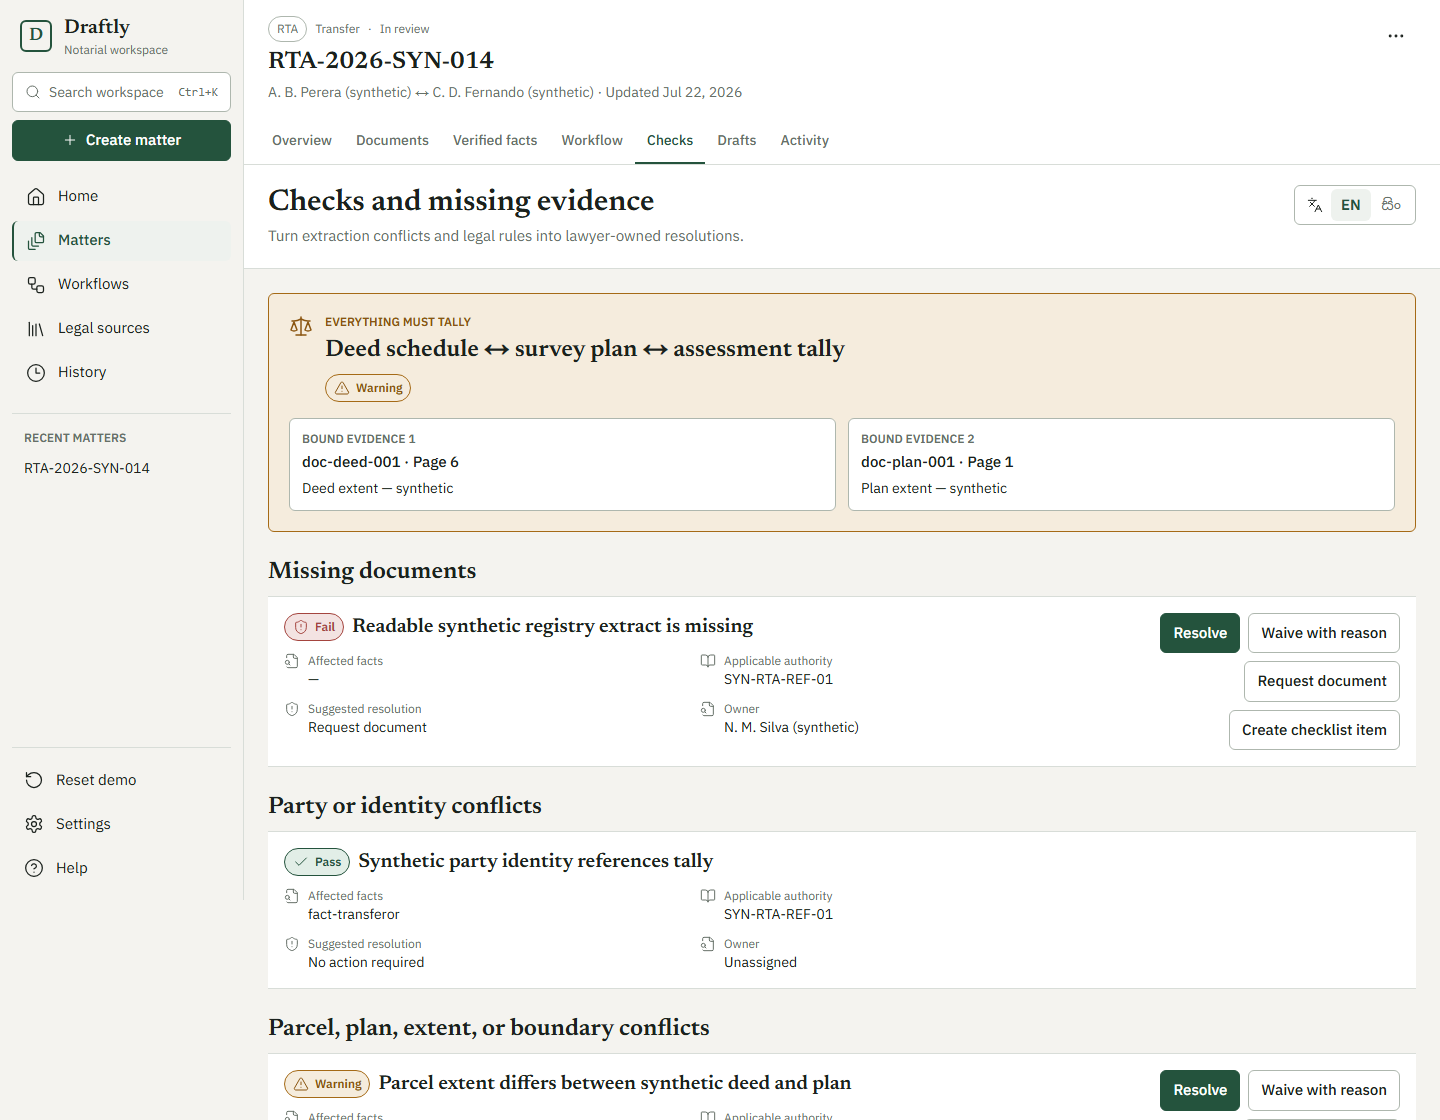
\includegraphics[width=\linewidth,height=5in,keepaspectratio]{figures/ui-prototype-checks.png}
\caption{Checks prototype with synthetic matter data, captured 22 July 2026. Findings require a lawyer-owned response.}
\end{figure}

The implemented research view returns cited passages or an explicit insufficient-authority state. Draft screens show form bindings and unresolved values for lawyer review. The workflow records preflight decisions, approvals, and export events, with refusal tests covering missing prerequisites.


\section{System Testing and Analysis}

\subsection{Testing Approach}

Testing targeted each rule at the layer that enforces it. Domain policies were unit-tested, repositories and service transactions were tested against PostgreSQL, and route sweeps checked organisation isolation, concurrency conditions and API conventions. The frontend logic and components were tested with Vitest; browser tests exercised selected refusal behaviour with Playwright. Synthetic data was used throughout. The platform test report records the scope and deviations: full authenticated browser journeys, load and failover tests, external paid-service runs, and lawyer acceptance tests were not completed in that cycle. The tested browser journey concentrated on refusal behaviour at drafting and approval gates.


\subsection{Platform Test Results}

The dated backend and frontend runs on 19 September 2026 collected 3,922 backend tests, of which 3,906 passed, ten were expected failures, one was skipped, and five live-service tests were excluded. All 348 frontend unit and component tests passed. Three refusal tests covering one browser journey passed. These figures do not mean that the entire browser suite passed: the separate 20 September single-worker run recorded four passed, nine failed and two skipped across the older and new browser tests. Table 3 keeps the results and coverage boundaries separate.


\begin{table}[H]
\centering
\caption{Platform test execution and coverage recorded in September 2026.}
\fontsize{9.5}{11}\selectfont
\begin{tabularx}{\linewidth}{>{\RaggedRight\arraybackslash}X|>{\RaggedRight\arraybackslash}X|>{\RaggedRight\arraybackslash}X}
\toprule
\textbf{Measure} & \textbf{Recorded result} & \textbf{Interpretation} \\
\midrule
Backend pytest & 3,906 passed; 0 failed; 10 expected failures; 1 skipped; 5 live tests excluded & Real PostgreSQL used for database and security suites \\
Frontend Vitest & 348 passed & Logic-layer coverage 93.3\%; whole frontend line coverage 27.0\% \\
Browser refusal tests & 3 passed for one journey & Whole browser suite had other failures and was not in CI \\
Backend coverage & 85.4\% lines; 63.9\% branches & Line target met; branch target of 70\% not met \\
Defects found and fixed & 15, including 2 critical & 12 appeared only with real PostgreSQL behaviour \\
\bottomrule
\end{tabularx}
\end{table}

The seven named safety rules were traced to passing tests: cross-organisation isolation, material-action audit, privacy of client identifiers at rest, role and capability enforcement, consistent API behaviour, reliable outbox delivery, and quota accounting. A forged pagination cursor and malformed webhook were also tested as refusals. Hash-chain concurrency testing found and fixed a case in which two writers could fork an audit log. These results support the tested security, persistence, audit, and workflow behaviour of the workbench.


\subsection{Performance, Security and Failure Behaviour}

On the research laptop, the BM25 retrieval baseline took about 16 ms per query, hybrid fusion 17 ms, the structure-aware system about 0.9 s, and the cross-encoder variant about 6.8 s. These are experiment measurements on a fixed corpus and processor, not end-to-end response times of the deployed web application. The deployment record describes a single virtual private server and a lexical retrieval index. If that service is unreachable, the research path returns insufficient authority. The same record states that document extraction is stubbed and real-client use is not yet approved. The platform test plan included load, failover and real-client use only as later work.


\subsection{Evaluation of Machine Learning and Data Science Components}

Retrieval was scored on 40 test questions grouped into 32 matters. Indispensable recall at 20, R@20, averages the fraction of each question's indispensable sections retrieved. Complete-indispensable recall at 20, C@20, credits a question only when all of its indispensable sections appear in the first 20 results. Question scores were averaged within each matter and then across matters; 95 percent intervals used 2,000 matter-level bootstrap resamples. All labels are agent-produced proposed gold and remain subject to attorney review. Table 4 reports the seven main systems.


\begin{table}[H]
\centering
\caption{Main-test retrieval results (matter-macro means; proposed labels).}
\fontsize{8.5}{10}\selectfont
\begin{tabularx}{\linewidth}{>{\RaggedRight\arraybackslash}X|>{\RaggedRight\arraybackslash}X|>{\RaggedRight\arraybackslash}X|>{\RaggedRight\arraybackslash}X|>{\RaggedRight\arraybackslash}X|>{\RaggedRight\arraybackslash}X}
\toprule
\textbf{System} & \textbf{R@20} & \textbf{C@10} & \textbf{C@20} & \textbf{MRR} & \textbf{Act@10} \\
\midrule
BM25 & 0.491 & 0.250 & 0.281 & 0.503 & 0.719 \\
Field-weighted BM25 & 0.482 & 0.250 & 0.281 & 0.540 & 0.672 \\
Dense BGE & 0.379 & 0.125 & 0.188 & 0.316 & 0.562 \\
Hybrid rank fusion & 0.546 & 0.266 & 0.344 & 0.543 & 0.625 \\
Hybrid plus cross-encoder & 0.413 & 0.125 & 0.234 & 0.223 & 0.562 \\
Hierarchical & 0.496 & 0.297 & 0.375 & 0.509 & 0.469 \\
Hierarchical plus typed expansion & 0.480 & 0.281 & 0.312 & 0.495 & 0.469 \\
\bottomrule
\end{tabularx}
\end{table}

\begin{figure}[H]
\centering
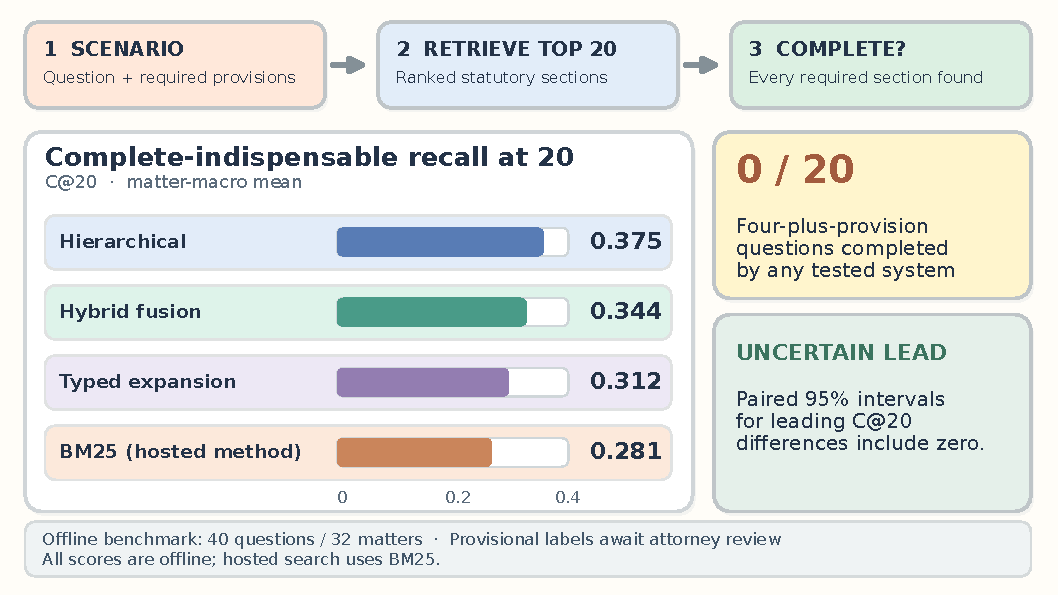
\includegraphics[width=\linewidth,keepaspectratio]{figures/report-fig-13-retrieval-c20-comparison.pdf}
\caption{Complete-indispensable recall at 20 for four systems from Table 4 (40 test questions in 32 matters; matter-macro means; proposed labels pending attorney review). All scores are from the offline benchmark; hosted search uses BM25. The leading pairwise C@20 intervals include zero.}
\end{figure}

Hybrid fusion produced the highest R@20 and MRR, whereas hierarchical retrieval had the highest observed C@20 and BM25 had the highest Act@10. Fig. 13 compares the four C@20 point estimates. The paired C@20 differences among hybrid, hierarchical and structure-aware retrieval were uncertain on this small test split; the structure-aware minus hybrid difference was −0.031 with a 95 percent interval from −0.156 to +0.078. The cross-encoder variant reduced MRR from 0.543 to 0.223. The structure-aware temporal filter removed out-of-force sections from its top ten results, while the flat systems retained some; this is a tested filtering result rather than a claim that all historical law is represented perfectly. Fig. 14 shows why aggregate recall hides the hardest questions: no system completed any of the 20 test questions requiring four or more indispensable sections.


\begin{figure}[H]
\centering
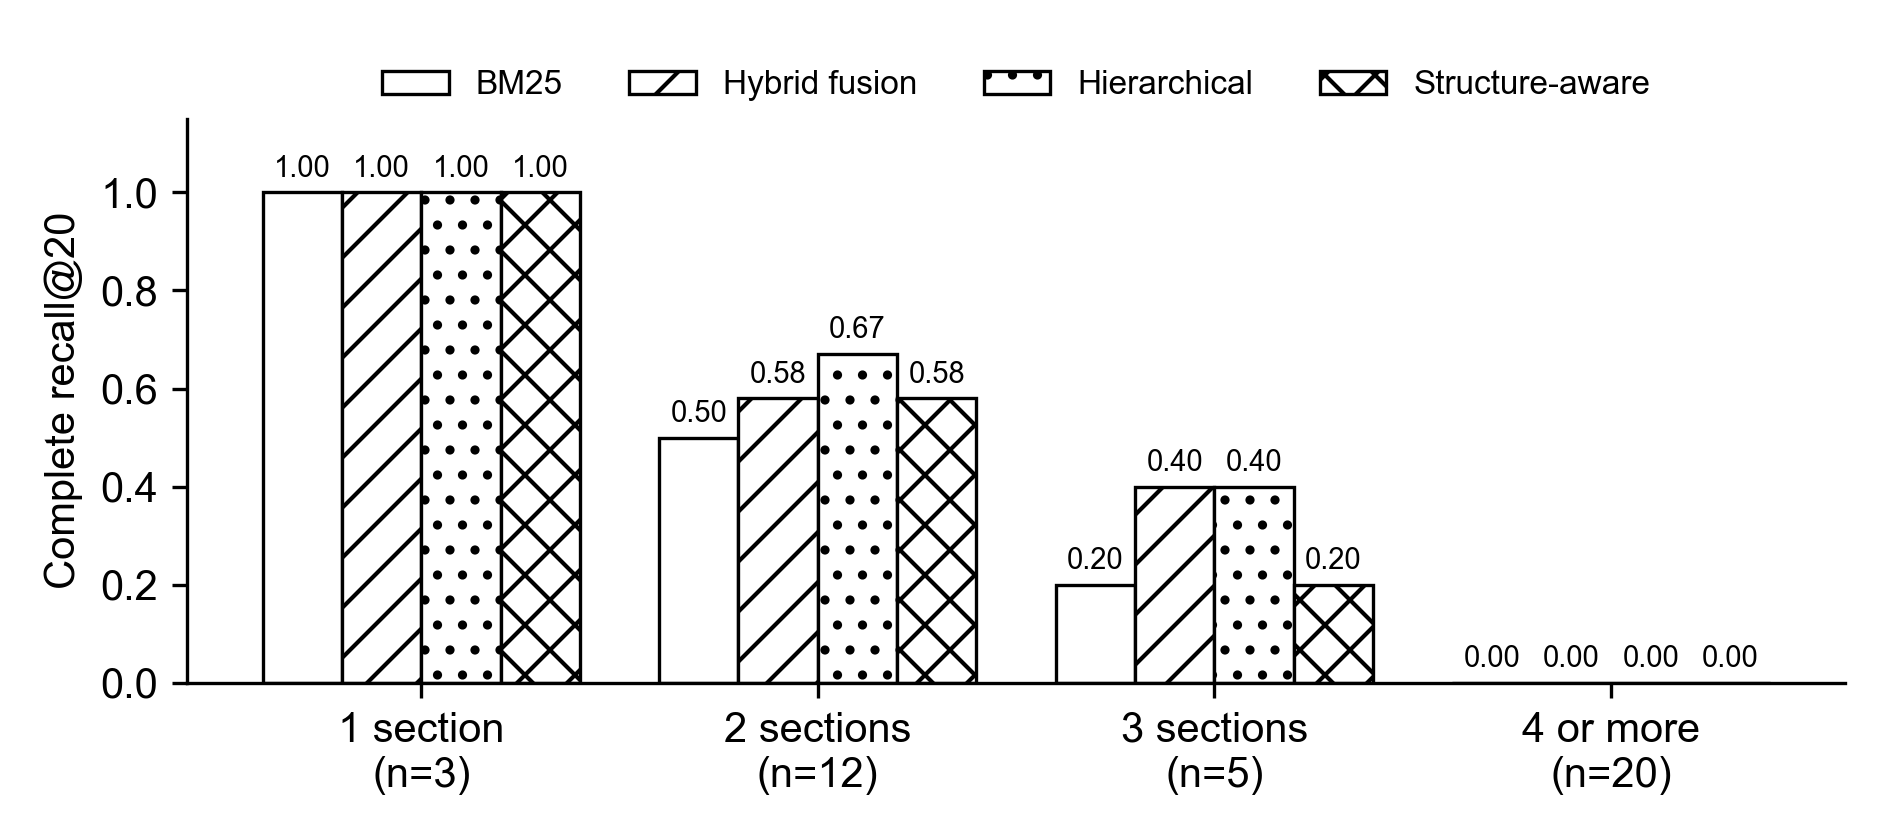
\includegraphics[width=\linewidth,height=5in,keepaspectratio]{figures/report-fig-13-recall-by-bundle-size.png}
\caption{C@20 by the number of indispensable sections on the 40-question test split; all provision labels are provisional.}
\end{figure}

Only two of the 114 indispensable sections missed by the structure-aware system were reachable by a single typed edge from a retrieved seed. The graph therefore lacks most of the dependencies a complete answer needs, even when its edges are valid descriptions of explicit textual relationships. Scenarios enriched with relevant conditions scored better than the original wording, which suggests that identifying legally operative facts may matter more than adding more of the same one-hop edges. This remains a research inference, not a proven improvement in the deployed platform.


The case-law extraction study accepted 74 of 100 held-out cases under the quote-grounding gate. A language-model judge, used only as a provisional proxy, rated 58.1 percent of those accepted rules fully usable, below the pre-registered 90 percent threshold. No extracted rule has been signed off by a lawyer. The multilingual OCR comparison informed the design choice, but the field-level extraction experiment could not be scored after paid runs failed on credentials. Accordingly, this report makes no field-accuracy claim. Answer generation itself has not been graded for legal correctness. These gaps define the boundary of the evaluation rather than being filled with assumptions from a working interface.


\section{Conclusion and Future Work}

Draftly addressed a practical conveyancing problem: a lawyer must reconcile evidence and find the complete, applicable legal authority before making a professional decision. The project produced a structured statutory corpus and a provisional scenario benchmark, tested seven retrieval systems, and built a matter-centred workbench that keeps candidates, citations, checks and human decisions separate. The measured retrieval result was mixed. Hybrid fusion improved average indispensable recall, hierarchical retrieval recorded the highest observed complete recall, and the tested typed-edge expansion did not improve completeness. Most missed provisions lacked an explicit one-hop relationship to a retrieved seed. Temporal filtering removed out-of-force sections in the tested ranking, while no system completed a question needing four or more provisions.


The platform demonstrates a persistent, lawyer-controlled matter workflow. PostgreSQL tests exercised access control, audit, privacy, concurrency, and refusal gates; the hosted system connects the interface, API, database, worker, and internal legal search. The next evaluation phase will bring practising lawyers into benchmark adjudication, document-field assessment, and form review. It will also test dense retrieval in deployment and complete authenticated browser journeys across drafting and approval.


\clearpage
\section*{References}
\addcontentsline{toc}{section}{References}

\begingroup
\small
\setlength{\parindent}{0pt}
\setlength{\parskip}{4pt}

\hangindent=0.35in \hangafter=1 \textnormal{[1]} Registration of Title Act, No. 21 of 1998, Parliament of the Democratic Socialist Republic of Sri Lanka, 1998.\par

\hangindent=0.35in \hangafter=1 \textnormal{[2]} H. Dhanapala, L. Dilshan, P. de Silva, and N. de Silva, "Does statutory structure help? Retrieving every indispensable provision for Sri Lankan conveyancing scenarios," accepted for presentation at the GlobalSouthAI Workshop, 40th Conf. Neural Inf. Process. Syst. (NeurIPS), 2026.\par

\hangindent=0.35in \hangafter=1 \textnormal{[3]} S. Paul, D. Ghumare, P. Goyal, S. Ghosh, and A. Modi, "IL-PCSR: Legal corpus for prior case and statute retrieval," in Proc. 2025 Conf. Empirical Methods Natural Lang. Process. (EMNLP), 2025, pp. 14588–14611.\par

\hangindent=0.35in \hangafter=1 \textnormal{[4]} N. Pipitone and G. H. Alami, "LegalBench-RAG: A benchmark for retrieval-augmented generation in the legal domain," arXiv:2408.10343, 2024.\par

\hangindent=0.35in \hangafter=1 \textnormal{[5]} L. Zheng, N. Guha, J. Arifov, S. Zhang, M. Skreta, C. D. Manning, P. Henderson, and D. E. Ho, "A reasoning-focused legal retrieval benchmark," in Proc. 2025 Symp. Comput. Sci. Law (CS\&Law), 2025.\par

\hangindent=0.35in \hangafter=1 \textnormal{[6]} J. Lee, D. Kim, S. Hwang, H. Kim, and G. Lee, "KoBLEX: Open legal question answering with multi-hop reasoning," in Proc. 2025 Conf. Empirical Methods Natural Lang. Process. (EMNLP), Suzhou, China, 2025, pp. 4019–4053.\par

\hangindent=0.35in \hangafter=1 \textnormal{[7]} E. Beta, O. S. Chlapanis, D. Galanis, and I. Androutsopoulos, "GreekBarRetrieval: A benchmark for Greek statutory retrieval," arXiv:2608.18752, 2026.\par

\hangindent=0.35in \hangafter=1 \textnormal{[8]} K. Chae et al., "Evaluating structure-aware retrieval and safety in statute-centric legal QA," in Proc. 64th Annu. Meeting Assoc. Comput. Linguistics (ACL), San Diego, CA, USA, 2026, pp. 45553–45573.\par

\hangindent=0.35in \hangafter=1 \textnormal{[9]} M. Prior, A. Schultz, and M. Grabmair, "Asking for an old friend: Diagnosing and mitigating temporal failure modes in LLM-based statutory question answering," arXiv:2605.23497, 2026.\par

\hangindent=0.35in \hangafter=1 \textnormal{[10]} O. Atukorala, R. Appuhami, and N. de Silva, "LawChain: A resource-efficient blueprint for legal information retrieval in low-resource jurisdictions," in GlobalSouthML Affinity Workshop, 43rd Int. Conf. Mach. Learn. (ICML), San Diego, CA, USA, 2026. [Online]. Available: https://icml.cc/virtual/2026/78334\par

\hangindent=0.35in \hangafter=1 \textnormal{[11]} A. Athulathmudali, "AI for legal domain identification and guidance in Sri Lankan law," Int. J. Innov. Sci. Res. Technol., vol. 10, no. 12, pp. 609–621, 2025, doi: 10.38124/ijisrt/25dec441.\par

\hangindent=0.35in \hangafter=1 \textnormal{[12]} L. Jayawardena, N. Wiratunga, R. Abeyratne, K. Martin, I. Nkisi-Orji, and R. Weerasinghe, "SCaLe-QA: Sri Lankan case law embeddings for legal QA," in Proc. SICSA Workshop Reasoning, Eval. Appl. Large Lang. Models (SICSA-REALLM), CEUR Workshop Proc., vol. 3822, Aberdeen, U.K., 2024, pp. 47–55.\par

\hangindent=0.35in \hangafter=1 \textnormal{[13]} S. Robertson and H. Zaragoza, "The probabilistic relevance framework: BM25 and beyond," Found. Trends Inf. Retr., vol. 3, no. 4, pp. 333–389, 2009.\par

\hangindent=0.35in \hangafter=1 \textnormal{[14]} S. Xiao, Z. Liu, P. Zhang, N. Muennighoff, D. Lian, and J.-Y. Nie, "C-Pack: Packed resources for general Chinese embeddings," in Proc. 47th Int. ACM SIGIR Conf. Res. Develop. Inf. Retr., 2024, pp. 641–649.\par

\hangindent=0.35in \hangafter=1 \textnormal{[15]} G. V. Cormack, C. L. A. Clarke, and S. Buettcher, "Reciprocal rank fusion outperforms Condorcet and individual rank learning methods," in Proc. 32nd Int. ACM SIGIR Conf. Res. Develop. Inf. Retr., 2009, pp. 758–759.\par

\hangindent=0.35in \hangafter=1 \textnormal{[16]} W. Wang, F. Wei, L. Dong, H. Bao, N. Yang, and M. Zhou, "MiniLM: Deep self-attention distillation for task-agnostic compression of pre-trained transformers," in Adv. Neural Inf. Process. Syst. (NeurIPS), vol. 33, 2020.\par

\hangindent=0.35in \hangafter=1 \textnormal{[17]} N. Reimers and I. Gurevych, "Sentence-BERT: Sentence embeddings using Siamese BERT-networks," in Proc. 2019 Conf. Empirical Methods Natural Lang. Process. and 9th Int. Joint Conf. Natural Lang. Process. (EMNLP-IJCNLP), 2019, pp. 3982–3992.\par

\hangindent=0.35in \hangafter=1 \textnormal{[18]} J. Choe, J. Kim, and W. Jung, "Hierarchical retrieval with evidence curation for open-domain financial question answering on standardized documents," in Findings Assoc. Comput. Linguistics: ACL 2025, Vienna, Austria, 2025, pp. 16663–16681.\par

\hangindent=0.35in \hangafter=1 \textnormal{[19]} Orbital, "AI drafts for title and survey review." [Online]. Available: \url{https://www.orbital.tech/blog/ai-drafts-for-title-survey} (Accessed on Sep. 29, 2026).\par

\hangindent=0.35in \hangafter=1 \textnormal{[20]} Clio, "Clio Draft: Draft and manage documents." [Online]. Available: \url{https://help.clio.com/hc/en-us/articles/24317070863899-Clio-Draft-Draft-and-Manage-Documents} (Accessed on Sep. 29, 2026).\par

\hangindent=0.35in \hangafter=1 \textnormal{[21]} Harvey, "Getting Started with Harvey." [Online]. Available: \url{https://help.harvey.ai/articles/getting-started-with-harvey} (Accessed on Sep. 29, 2026).\par

\hangindent=0.35in \hangafter=1 \textnormal{[22]} D. Hendrycks et al., "CUAD: An expert-annotated NLP dataset for legal contract review," in Proc. NeurIPS Datasets and Benchmarks, 2021. [Online]. Available: \url{https://www.atticusprojectai.org/cuad/}\par

\hangindent=0.35in \hangafter=1 \textnormal{[23]} Y. Koreeda and C. D. Manning, "ContractNLI: A dataset for document-level natural language inference for contracts," in Findings of EMNLP, 2021. [Online]. Available: \url{https://aclanthology.org/2021.findings-emnlp.164/}\par

\hangindent=0.35in \hangafter=1 \textnormal{[24]} A. B. Hou et al., "CLERC: A dataset for U. S. legal case retrieval and retrieval-augmented analysis generation," in Findings of NAACL, 2025. [Online]. Available: \url{https://aclanthology.org/2025.findings-naacl.441/}\par

\hangindent=0.35in \hangafter=1 \textnormal{[25]} D. Das et al., "LawFlow: Collecting and simulating lawyers' thought processes on business formation case studies," in Proc. Conf. Lang. Modeling (COLM), 2025. [Online]. Available: \url{https://openreview.net/pdf?id=MsgdEkcLRz}\par

\hangindent=0.35in \hangafter=1 \textnormal{[26]} M. Lasandi and N. Jayatilleke, "SinhaLegal: A benchmark corpus for information extraction and analysis in Sinhala legislative texts," arXiv:2603.04854, 2026. [Online]. Available: \url{https://arxiv.org/abs/2603.04854}\par

\hangindent=0.35in \hangafter=1 \textnormal{[27]} FastAPI. [Online]. Available: https://fastapi.tiangolo.com (Accessed on Sep. 28, 2026).\par

\hangindent=0.35in \hangafter=1 \textnormal{[28]} Next.js. [Online]. Available: https://nextjs.org (Accessed on Sep. 28, 2026).\par

\hangindent=0.35in \hangafter=1 \textnormal{[29]} PostgreSQL Global Development Group, PostgreSQL. [Online]. Available: https://www.postgresql.org (Accessed on Sep. 28, 2026).\par

\hangindent=0.35in \hangafter=1 \textnormal{[30]} Google Cloud, "Cloud Vision API." [Online]. Available: https://cloud.google.com/vision (Accessed on Sep. 28, 2026).\par

\hangindent=0.35in \hangafter=1 \textnormal{[31]} Google, "Gemini API." [Online]. Available: https://ai.google.dev (Accessed on Sep. 28, 2026).\par

\hangindent=0.35in \hangafter=1 \textnormal{[32]} Meta, "Llama 3.1 8B Instruct model card." [Online]. Available: https://huggingface.co/meta-llama/Llama-3.1-8B-Instruct (Accessed on Sep. 28, 2026).\par

\hangindent=0.35in \hangafter=1 \textnormal{[33]} NVIDIA, "NVIDIA NIM." [Online]. Available: https://build.nvidia.com (Accessed on Sep. 28, 2026).\par

\endgroup
\end{document}
